\documentclass[12pt]{report}
\usepackage[utf8]{inputenc}

\title{Base composition of Drosophila noncoding blocks and spacers}
\author{Manee Manee}
\date{June 2014}
\usepackage[pdftex]{graphicx} %
\usepackage{natbib} %
\usepackage{setspace} %
\usepackage{amssymb} %
\usepackage{anysize} %
\usepackage{courier} %
\usepackage{hyperref} %
\usepackage{subfigure} %
\marginsize{2.5cm}{3cm}{2.5cm}{2.5cm} %
\renewcommand{\thesection}{\arabic{section}} %
\setcounter{secnumdepth}{3} %
\setcounter{tocdepth}{3} %
\begin{document}
\pagestyle{plain} %
\maketitle
\onehalfspacing %
%\section{Introduction}

%\newpage
%\section{Project Objectives}

%\newpage
\section{Materials and Methods}
\subsection{Data sets}
PhastCons most conserved regions and exons data sets were downloaded from the UCSC Genome Browser database. Highly conserved elements (CEs) of D. melanogaster genomic loci (Tanay data set) were downloaded from the website of Amos Tanay group (\url{http://compgenomics.weizmann.ac.il/tanay/?page_id=459}) \citep{Tanay2013}.

\subsubsection{PhastCons elements}
PhastCons is a computer program, uses multiple alignment techniques to predict the CEs in different genomes. PhastCons elements represent the most conserved regions in vertebrate, insect, worm, and yeast genomes \citep{Siepel2005}. PhastCons program is based on a statistical model called a phylogenetic hidden Markov model (phylo-HMM). PhastCons program is a next-generation of computer program called VISTA, which considers two species genomes; and it is a part of a software package called PHAST (PHylogenetic Analysis with Space/Time models).

\subsubsection{Tanay elements}
Kenigsberg and Tanay identified approximately 67,780 CEs (average length of 50 bp), covering ~3\% of the \textit{D. melanogaster} genome \citep{Tanay2013}. Kenigsberg and Tanay demonstrated a new algorithm that learns evolutionary substitutions that are parameterized by flanking nucleotides. This algorithm executes a precise inference of ancestral divergence within a phylogenetic tree involving 12 \textit{Drosophila} species, and makes certain of correct control for substitution rates at high or low GC content sites. Kenigsberg and Tanay described conservation in genomes as neighbouring regions showing at two fold decrease in normalized divergence. 

\subsection{Generating block and spacer length distributions}
Distributions of phastCons and Tanay nonexonic CEs (blocks) lengths were generate. In addition, lengths between consecutive nonexonic conserved blocks (spacers) of phastCons and Tanay distributions were generated. The UCSC overlapSelect tool was used to filter out all phastCons most conserved regions that overlap exons to be able to generate a data set of nonexonic phastCons most conserved regions. Similarly, UCSC overlapSelect tool was used to filter out CEs of Tanay in order to generate data sets of nonexonic Tanay conserved block and spacer lengths. Length data sets of phastCons and Tanay conserved blocks and spacers were calculated and generated. Furthermore, data sets of exonic blocks, nonexonic blocks, exonic spacers, nonexonic spacers and exonic/nonexonic spacers were generated and plotted in order to compare between the two data sets of CEs (Figure 1).\\

\begin{figure}[htbp]
\centering
\frame{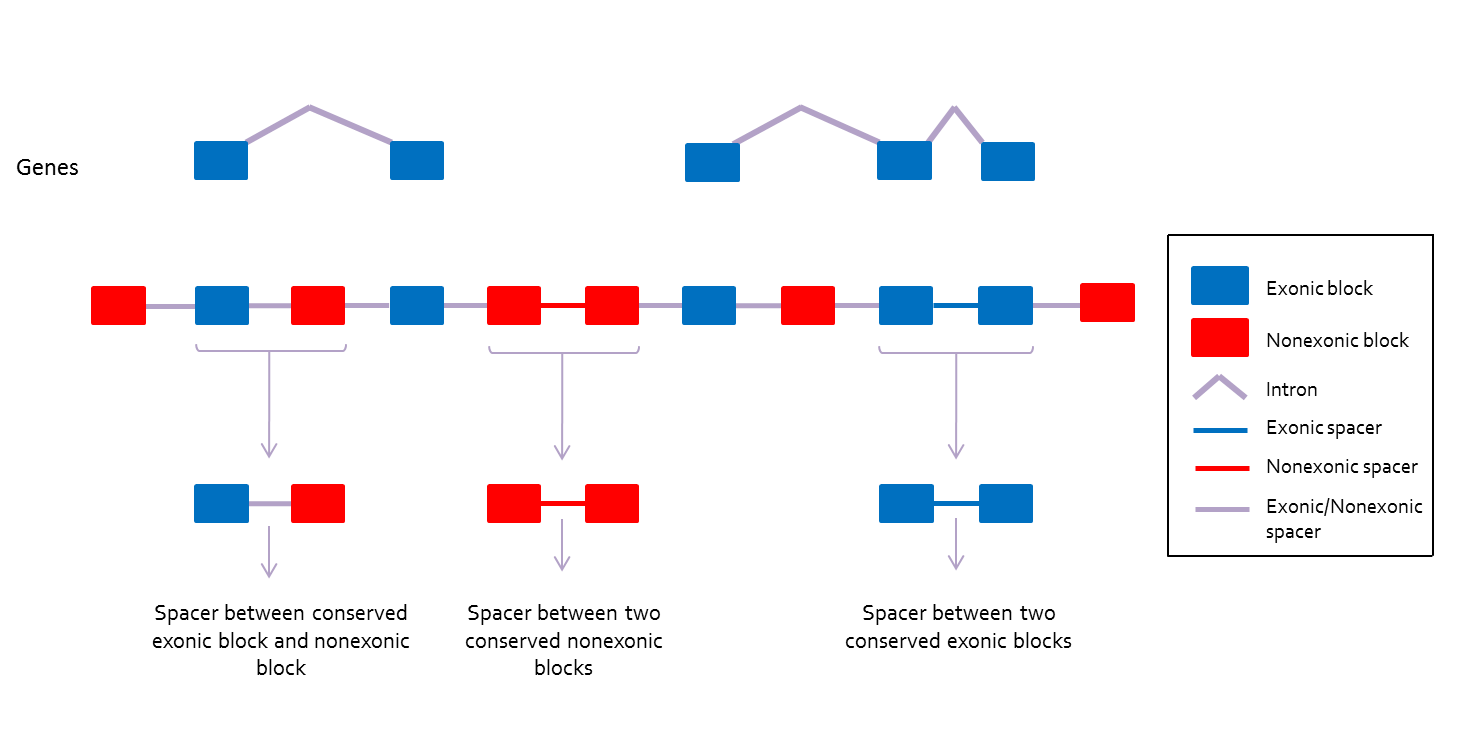
\includegraphics[width=120mm, height=75mm]{gene_structure.png}}
\caption{A schematic structure of multiple genes. A schematic of multiple exons above the schematic of blocks and spacers.}
\label{fig:gene_structure}
\end{figure}

\subsection{Performing overlap analysis of phastCons and Tanay blocks}
Overlap investigations were conducted to reveal the relationship between the phastCons and Tanay blocks. These investigations were performed to identify: (i) which Tanay blocks are in phastCons blocks and vice versa, (ii) how the two data sets overlap, are they overlap 1:1 or 1:Many (M), and (iii) for each block that overlaps in two data sets, determine which data set is bigger and how many additional base pairs are on 5' and 3' side of larger block. The overlap categories of phastCons (P) and Tanay (T) blocks include: (T1:P0), (T0:P1), (T1:P1), (T1:PM) and (TM:P1) (Figure 2).\\

\begin{figure}[htbp]
\centering
\frame{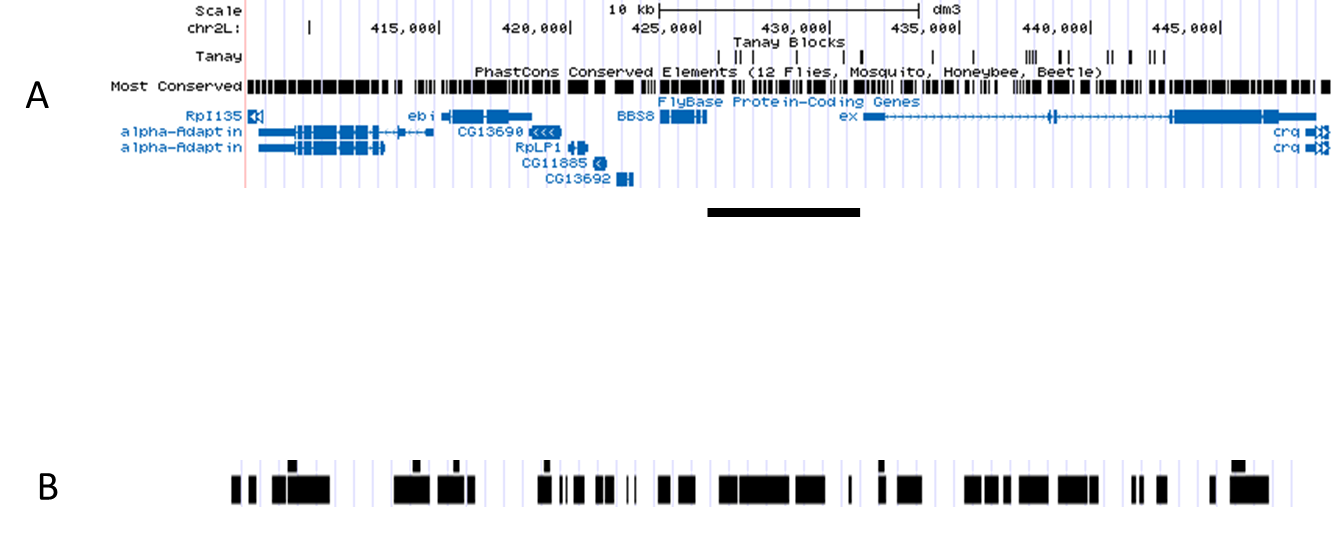
\includegraphics[width=\textwidth, height=65mm]{genome_browser.png}}
\caption[Caption for LOF]{Comparison of the phastCons and Tanay CEs. (A) Screen shot of a Genome Browser track shown that Tanay CEs overlap with phastCons CEs, and do not overlap with FlyBase Protein-Coding Genes. (B) the magnification of particular part of the Genome Browser track that includes a set of Tanay CEs that overlap with phastCons CEs}
\label{fig:tanay_phastCons}
\end{figure}

\begin{figure}[htbp]
\centering
\frame{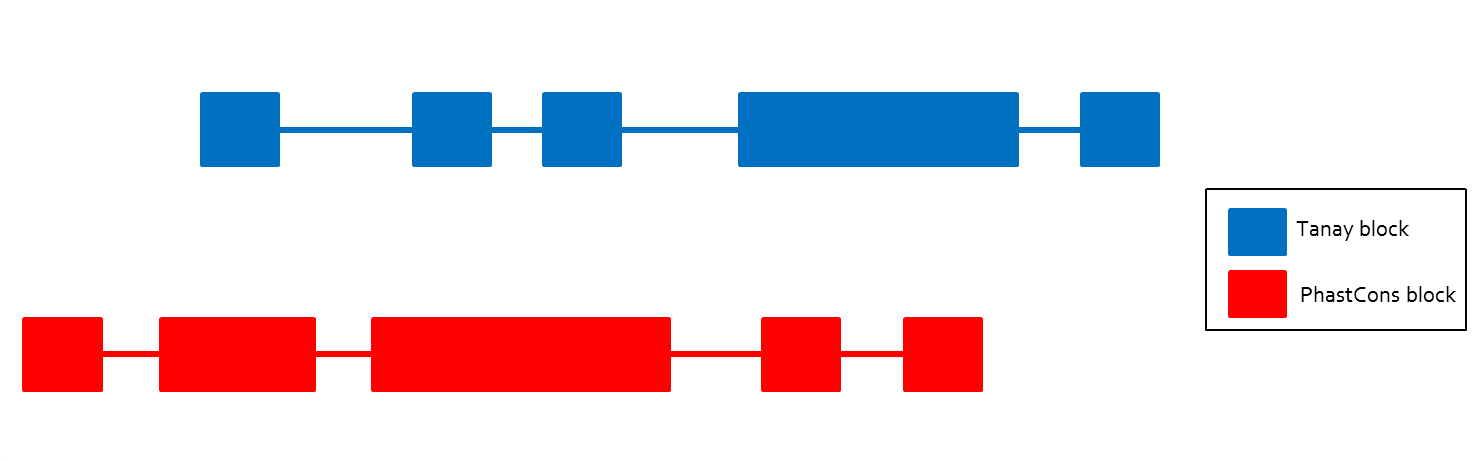
\includegraphics[width=140mm, height=45mm]{overlap.png}}
\caption{Overlap categories of phastCons and Tanay conserved blocks.}
\label{fig:T_P15_overlap}
\end{figure}

\subsection{Performing base composition analysis of phastCons and Tanay blocks and spacers}
Base composition investigations were performed to expose the fundamental features of sequences of phastCons and Tanay block and spacer. These investigations were conducted to determine: (i) base composition of phastCons and Tanay blocks, (ii) base composition of phastCons and Tanay spacers, (iii) base composition of the region in the larger block that is not present in the smaller overlapping block, and (iv) base composition of the overlapping region in phastCons and Tanay blocks. In addition, this study includes calculating AT content and GC content of phastCons and Tanay CEs, and regions flanking CEs.

\subsection{Investigating the relationship between base composition and block structure}
Previous analysis of GC content led to the conclusion that we needed to investigate the relationship between base composition and block length or position in block. This study assumes blocks identified independently of GC and that GC content is homogeneous within block. Subsequently, a number of questions remain unanswered need to be investigated: why is the GC profile not symmetrical, and how does block length affect GC-profile.

\newpage
\section{Results}
\subsection{Distributions of conserved block and spacer lengths}
Analysis of CEs of two data sets revealed that the data set of Tanay is very small in comparison with phastCons blocks. Investigation of length distributions of CEs showed that the length of Tanay blocks are short (average length of 50 bp). The notched box plots revealed the variability of the median number between the length of exonic and nonexonic blocks and spacers of phastCons and Tanay (Figure 3). The medians between the variables of two samples differ significantly.\\

\begin{figure}[htbp]
\centering
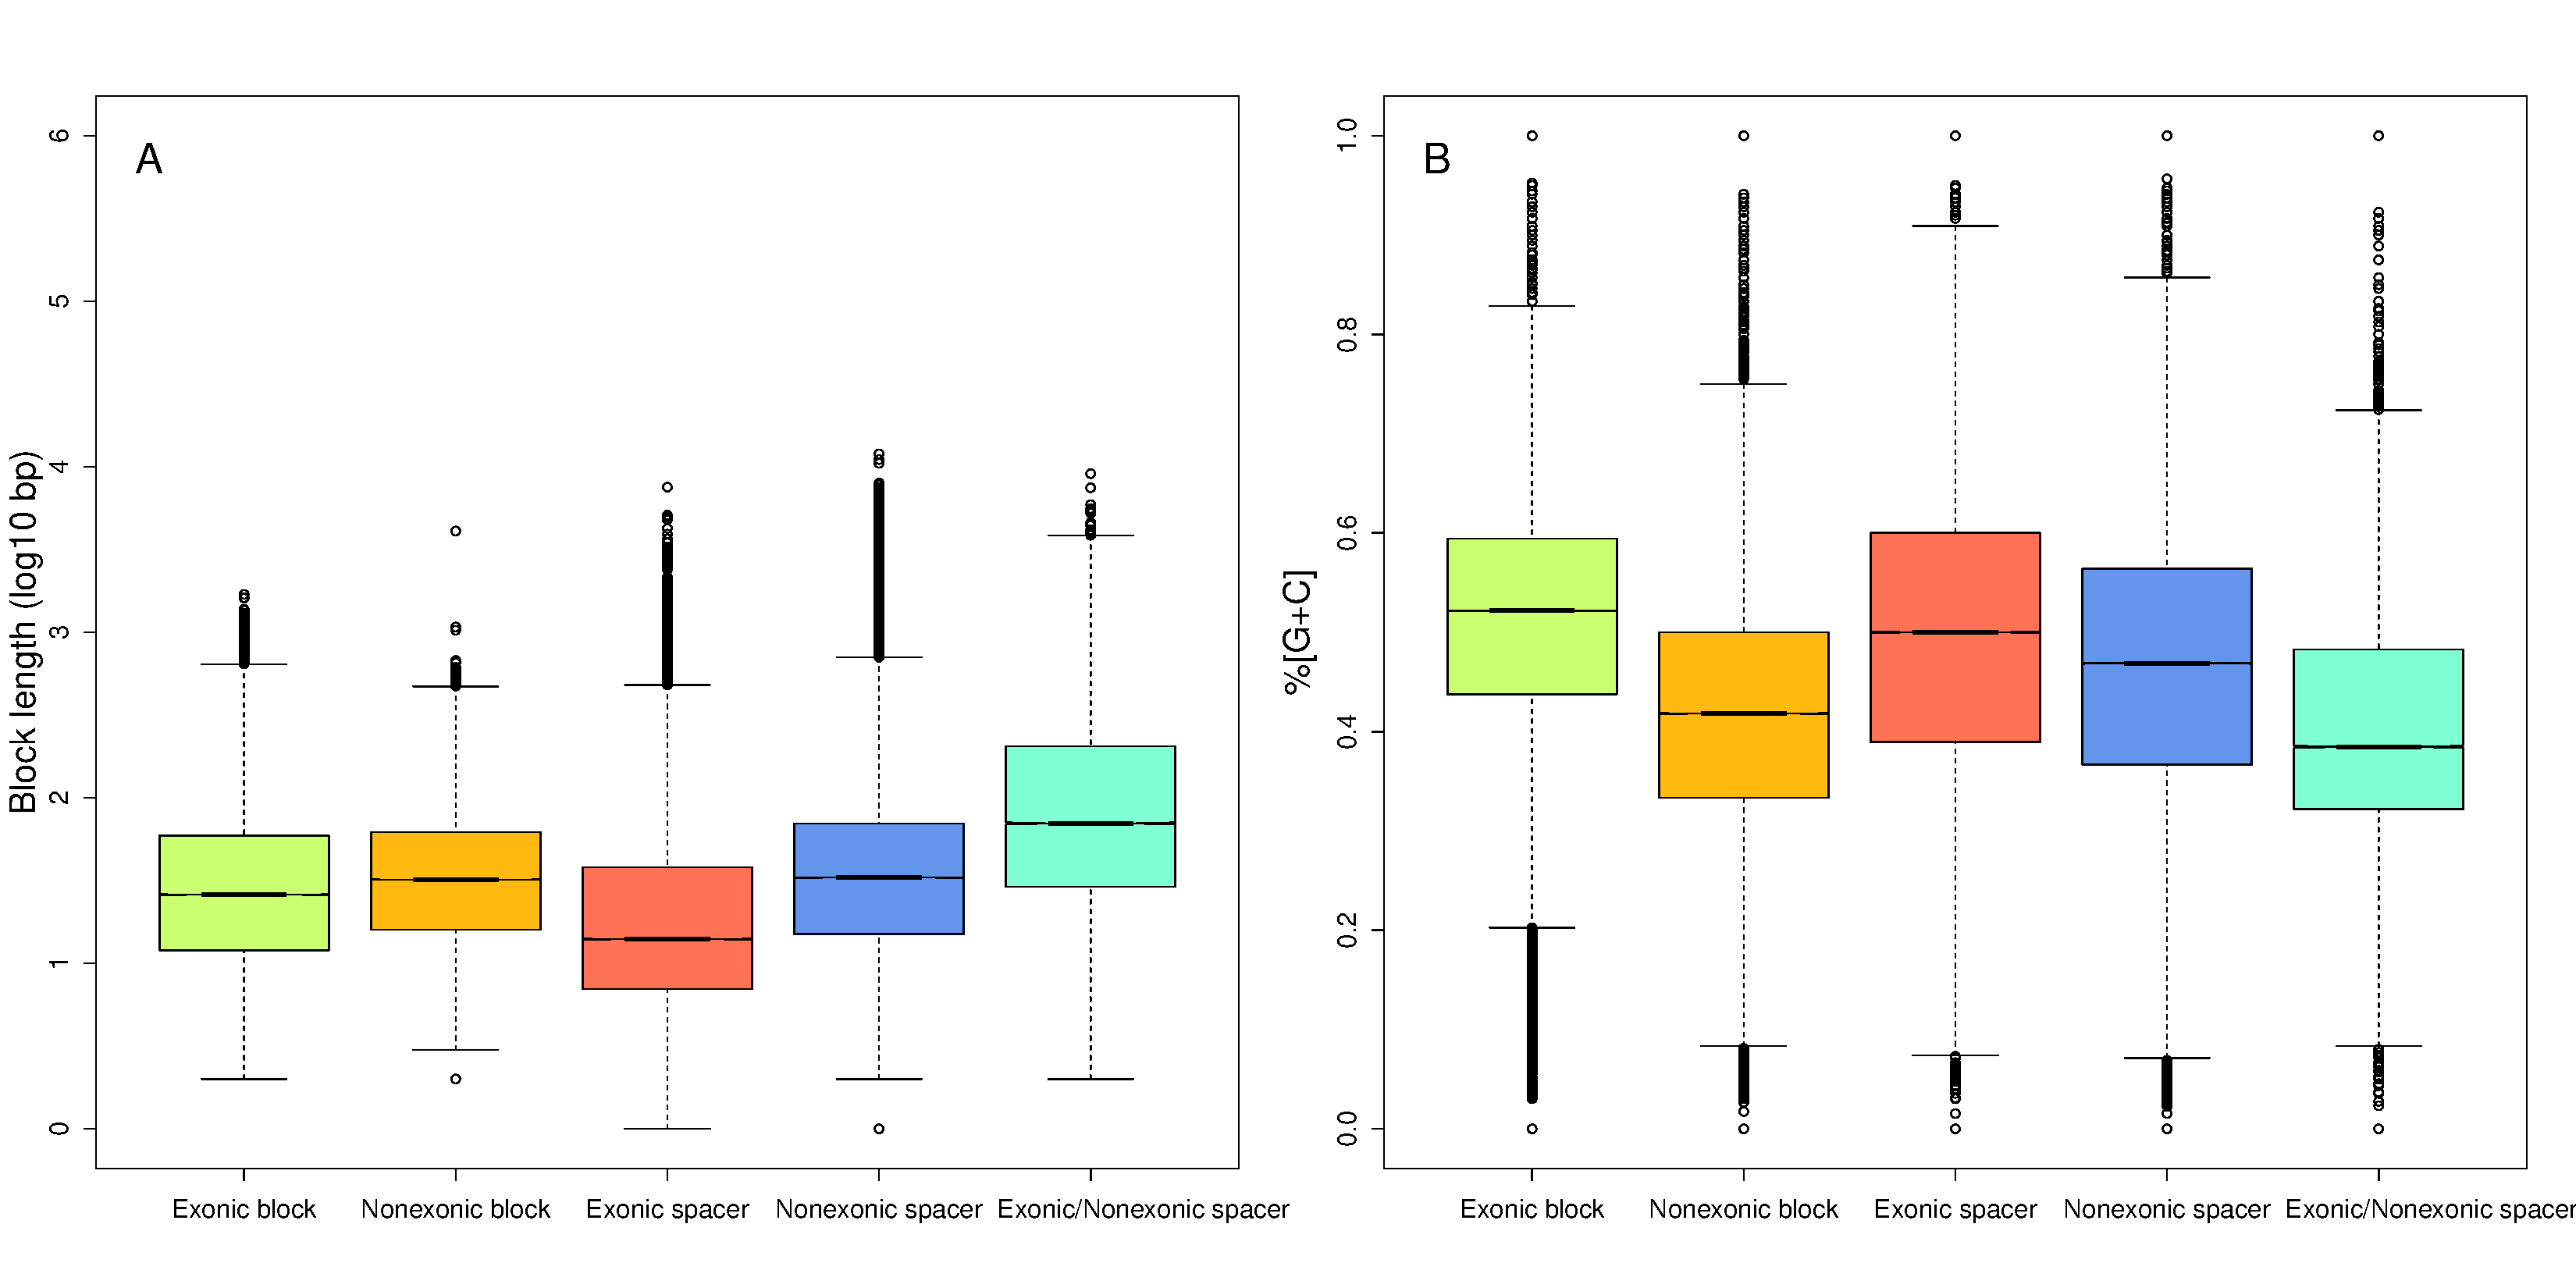
\includegraphics[width=\textwidth, height=82mm]{whole_phastcons_lenghts_GC_latex}
\caption{Length distributions (left panel) and average GC content (right panel) of complete phastCons data set.}
\label{fig:blocks_spacers_distributions_phast}
\end{figure}

\begin{table}[ht]
\centering
\begin{tabular}{c c c c}
\hline\hline
\ Category & Number & Average length (bp) & Average GC\% \\ [0.5ex]
\hline
Exonic blocks & 399551 & 47.9 & 0.510 \\
Nonexonic blocks & 674648 & 45.1 & 0.414 \\
Exonic spacers & 374993 & 35.5 & 0.502 \\
Nonexonic spacers & 650086 & 77.4 & 0.471 \\
Exonic/Nonexonic spacers & 49115 & 159.2 & 0.407 \\ [1ex] 
\hline
\end{tabular}
\caption[Caption for LOF]{\centering Average lengths and GC content of complete phastCons data set.}
\end{table}

\begin{figure}[htbp]
\centering
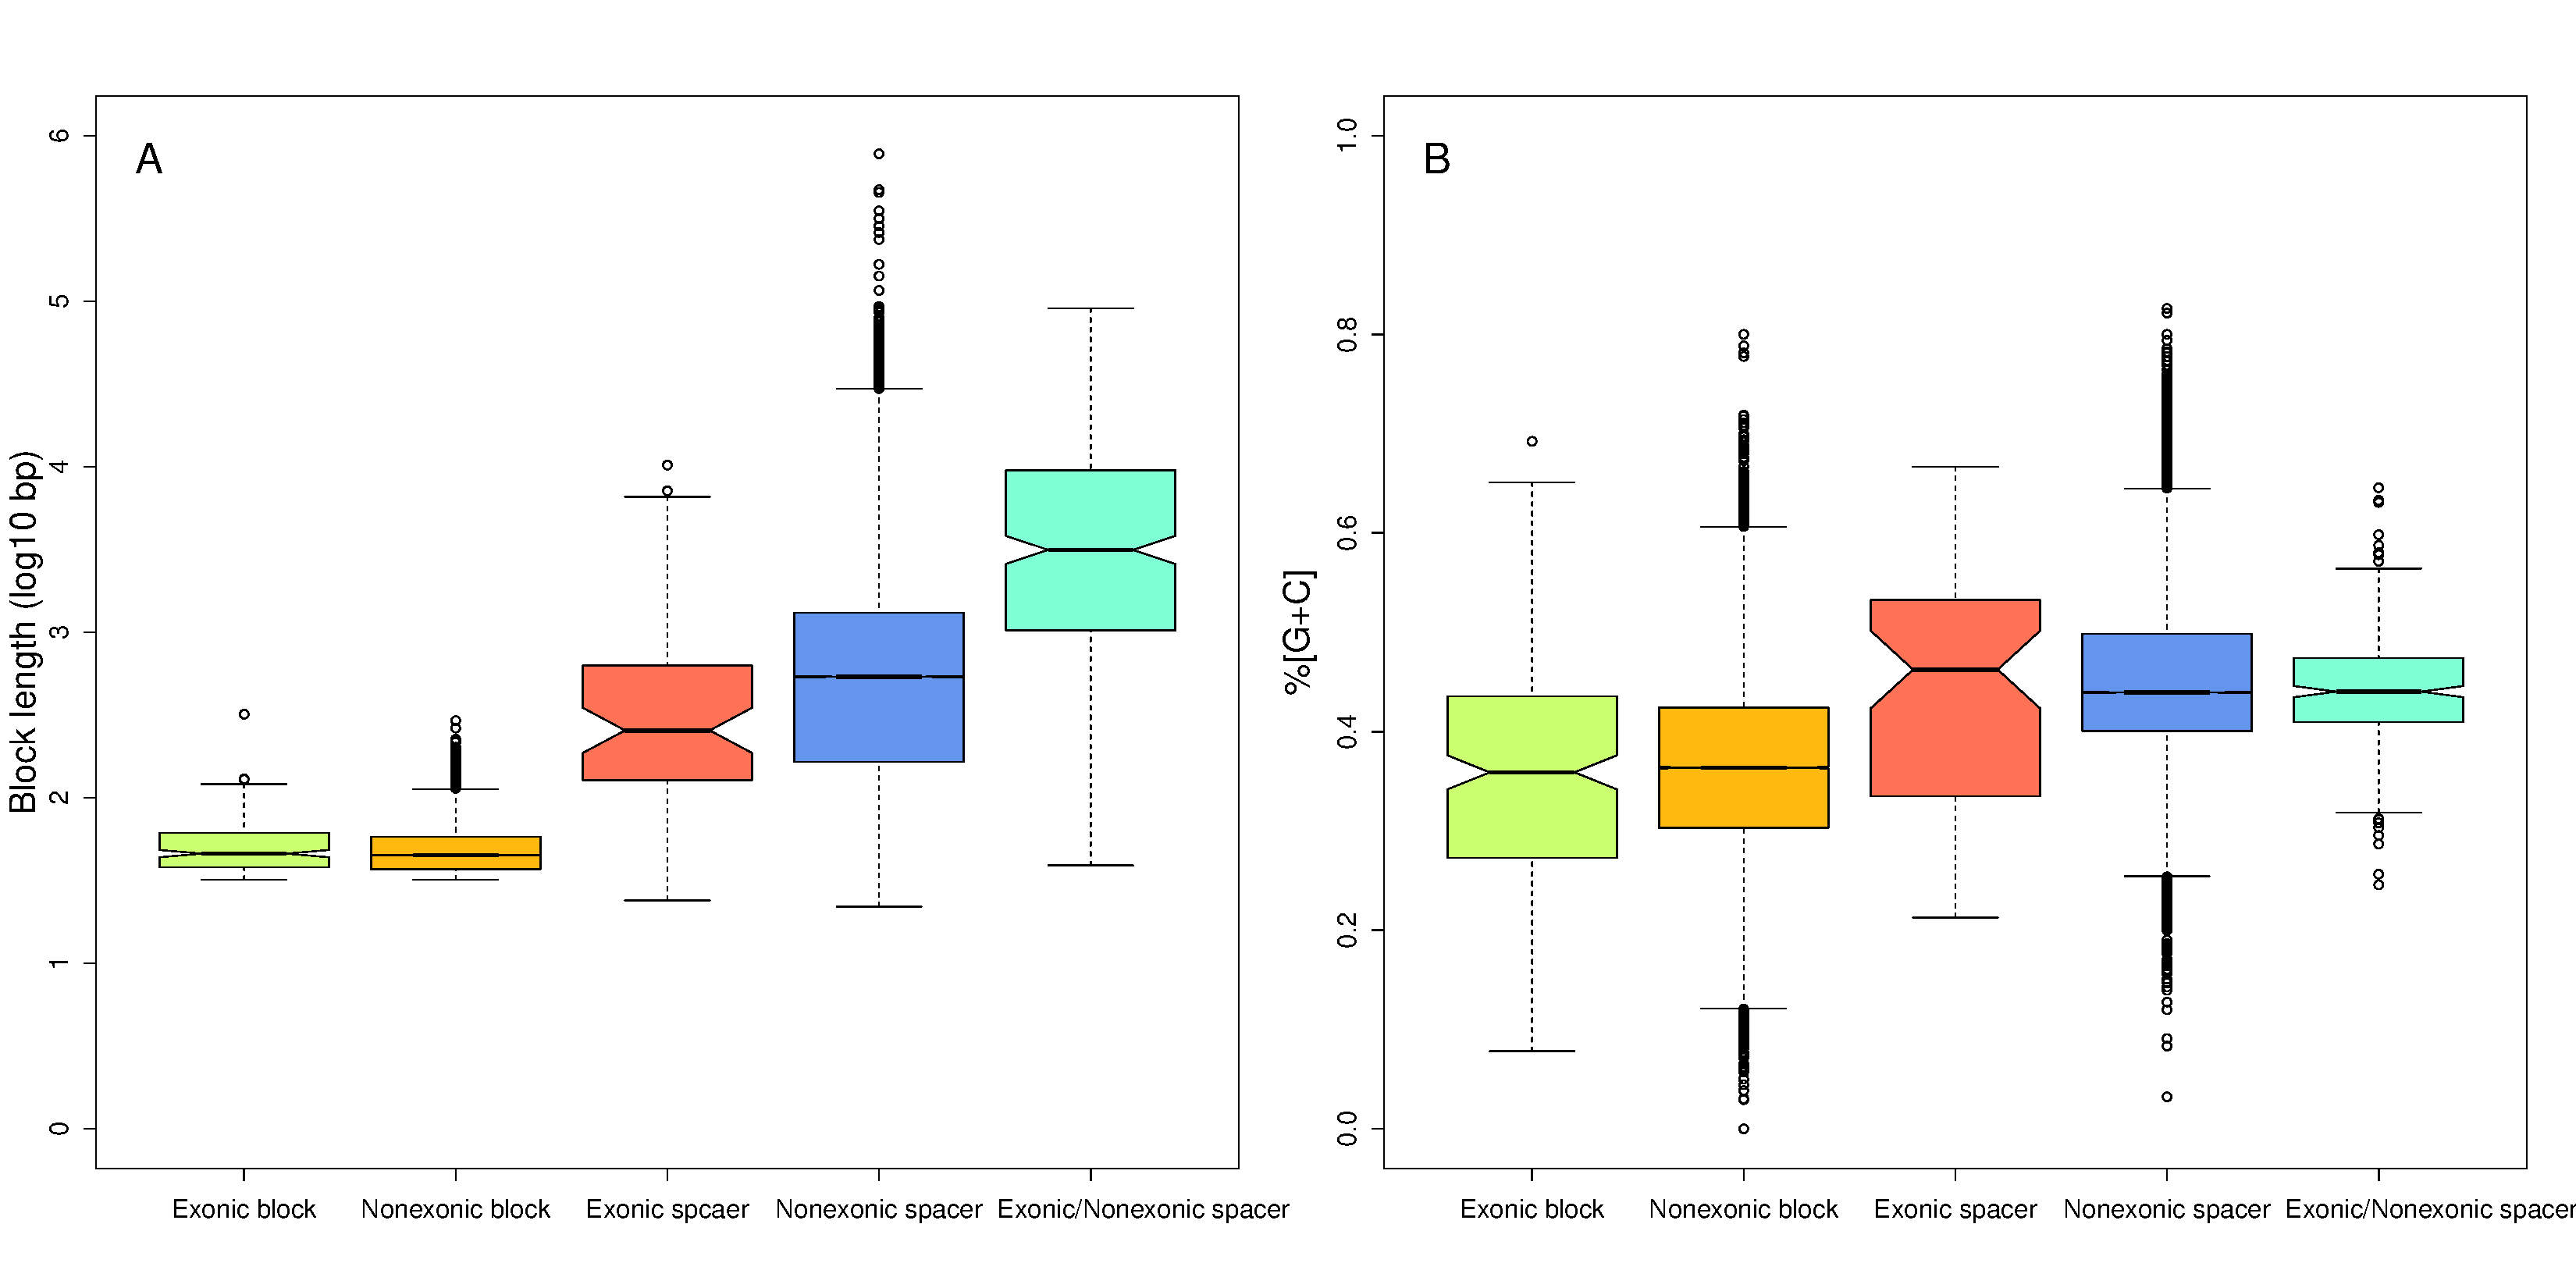
\includegraphics[width=\textwidth, height=82mm]{whole_tanay_lenghts_GC_latex}
\caption{Length distributions (left panel) and average GC content (right panel) of complete phastCons data set.}
\label{fig:blocks_spacers_distributions_tan}
\end{figure}

\begin{table}[ht]
\centering
\begin{tabular}{c c c c}
\hline\hline
\ Category & Number & Average length (bp) & Average GC\% \\ [0.5ex]
\hline
Exonic blocks & 227 & 49.9 & 0.359 \\
Nonexonic blocks & 67553 & 46.9 & 0.364 \\
Exonic spacers & 64 & 790.1 & 0.449 \\
Nonexonic spacers & 67385 & 1544.9 & 0.452 \\
Exonic/Nonexonic spacers & 326 & 7330.5 & 0.442 \\ [1ex] 
\hline
\end{tabular}
\caption[Caption for LOF]{\centering Average lengths and GC content of complete Tanay data set.}
\end{table}

\subsection{Overlap analysis of conserved blocks and spacers}
The vast majority of Tanay CEs are short. This was one motivation to conduct a comparison investigation between Tanay phastCons data sets. Most Tanay blocks were first submitted to UCSC Genome Browser, these blocks were found surprisingly to overlap with phastCons blocks (Figure 4). These observations led us to perform a comprehensive overlap study on CEs of Tanay and PhastCons. Using UCSC overlapSelect tool, 67775 conserved blocks of Tanay were found to overlap with phastCons blocks, and 66283 conserved blocks of phastCons were found to overlap with Tanay blocks. Only five CEs were excluded from Tanay data set. All overlap categories of phastCons and Tanay blocks were calculated and generated (see Table 1). The results of this study revealed that most Tanay blocks (94\%) are shown to have one-to-one overlap relationship (1:1) with phastCons blocks. This led us to focus on only analyzing the 1:1 overlap data set since this covers the vast majority of Tanay blocks.\\\\
Analysis of 1:1 data set showed that the frequency of occurrence by classes of blocks and spacers shows different distributions of PhastCopns and Tanay data sets (Figure 5). Moreover, average size of Tanay blocks is 47 bp, and 96 bp for phastCons blocks, covering in total 2.46\% and 5.03\% of the \textit{D. melanogaster} genome, respectively. The relationship study of 1:1 data set revealed that the size of almost all phastCons blocks is bigger than Tanay blocks (Figure 6). The interpretation of these results led to the conclusion that we required to perform a base composition study for Tanay and phastCons blocks and spacers.\\

\begin{table}[ht]
\centering
\begin{tabular}{c c c}
\hline\hline
\ Category & Tanay & PhastCons \\ [0.5ex]
\hline
Tanay 1 :PhastCons 0 & 5 & 0 \\
Tanay 0 :PhastCons 1 & 0 & 1152888 \\
Tanay 1 :PhastCons 1 & 64249 & 64249 \\
Tanay 1 :PhastCons M & 186 & 372 \\
Tanay M :PhastCons 1 & 3311 & 1634 \\ 
Tanay M :PhastCons M & 29 & 28 \\
\hline
Total & 67780 & 1219171 \\ [1ex]
\hline\hline
\end{tabular}
\caption[Caption for LOF]{\centering Overlap categories of phastCons and Tanay blocks}
\end{table}
 
\begin{figure}[htbp]
\centering
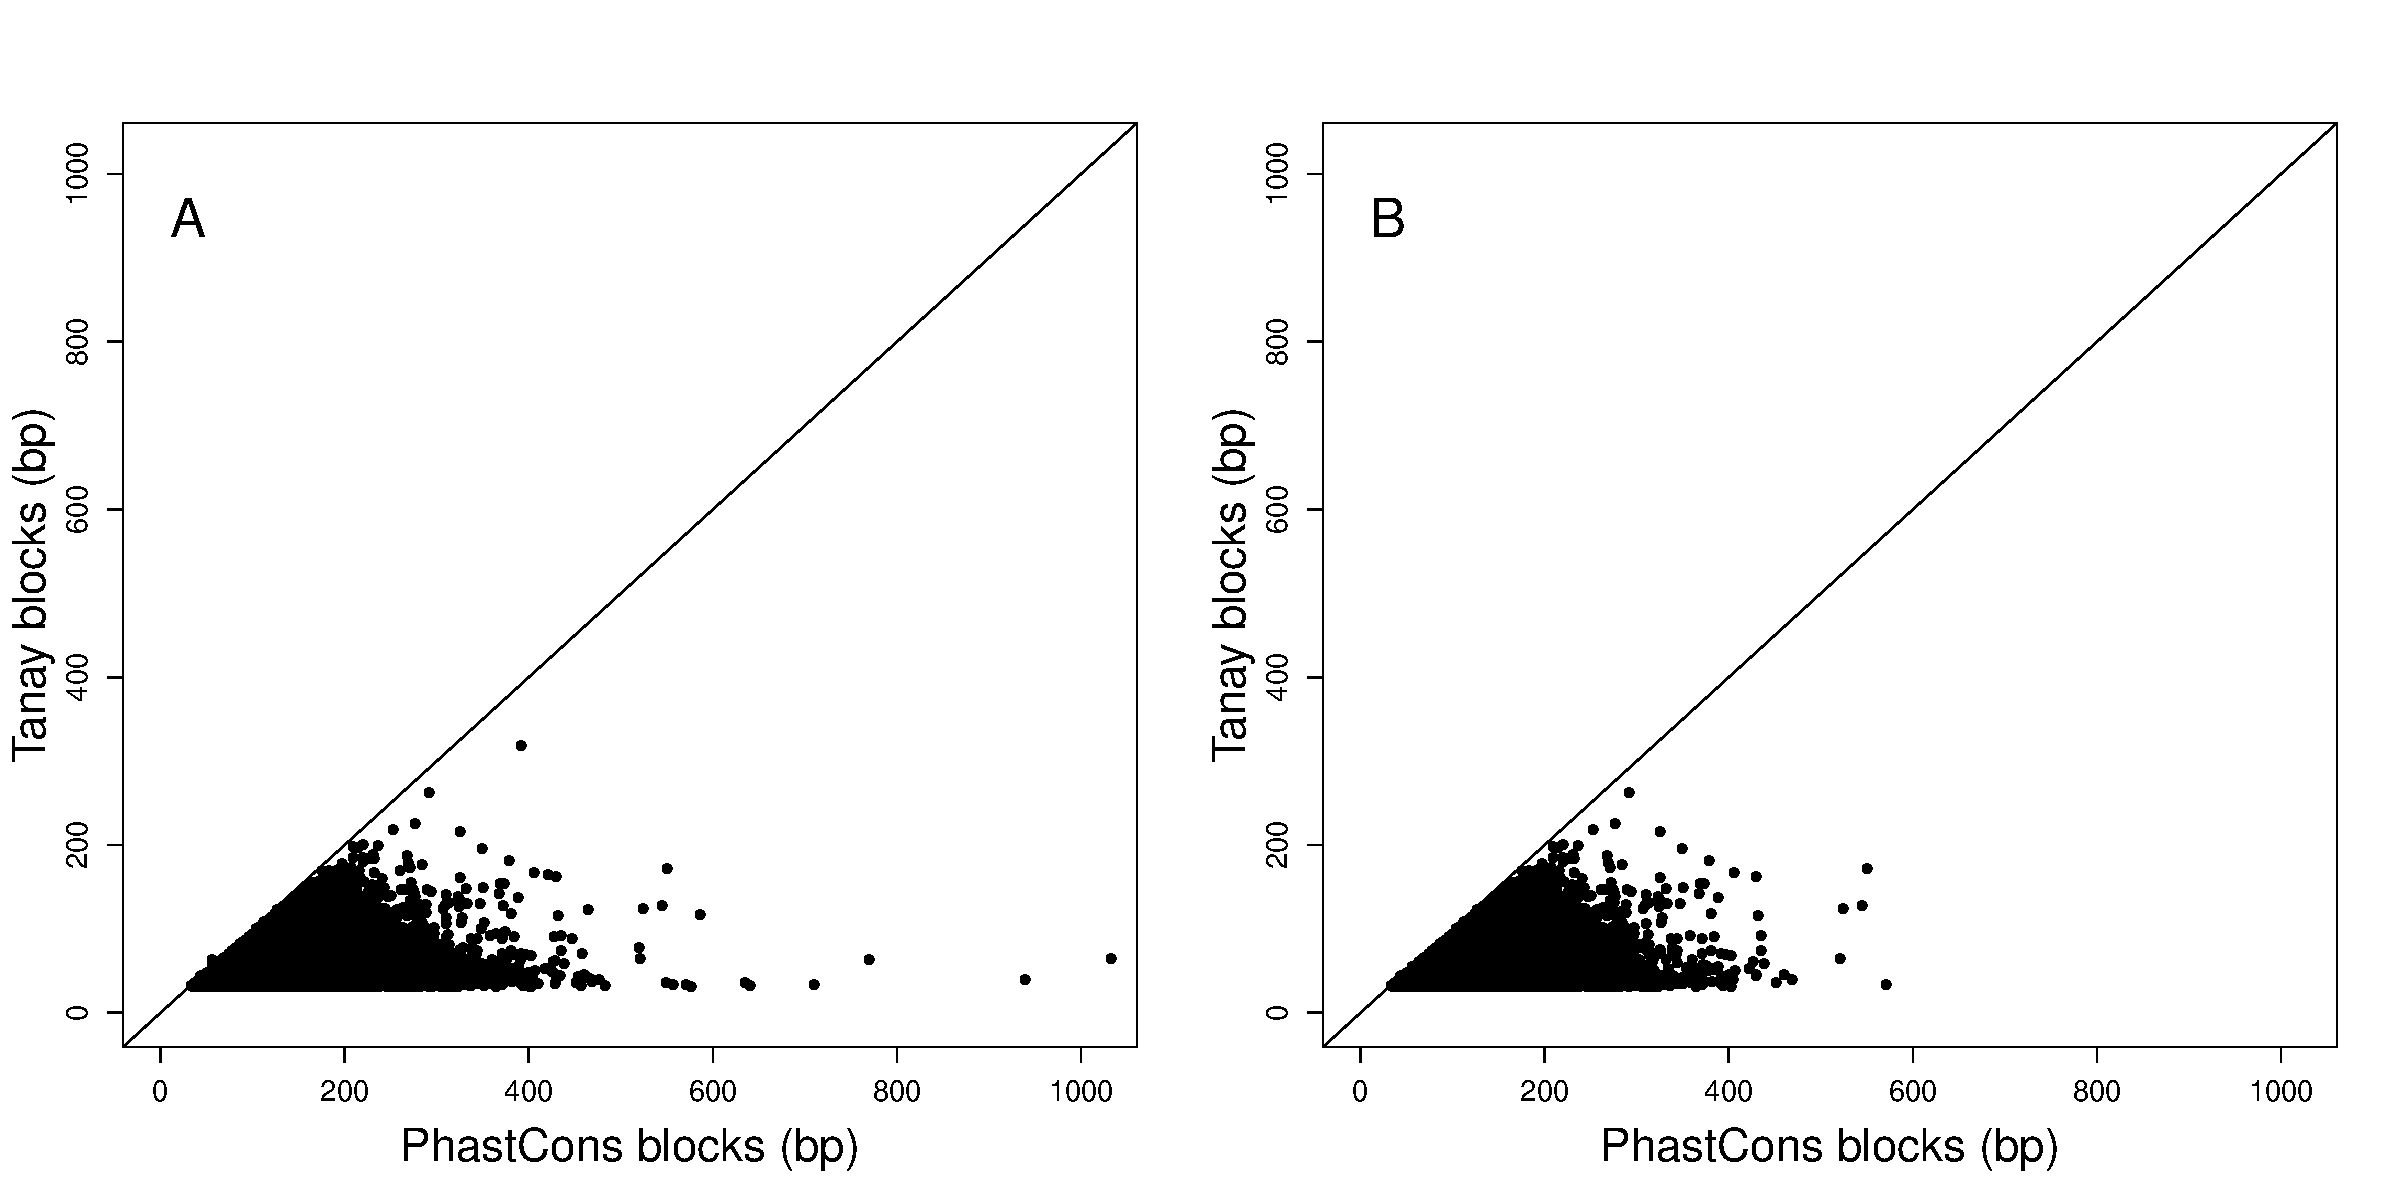
\includegraphics[width=\textwidth, height=80mm]{scatterplot_1_1_all_non}
\caption[Caption for LOF]{All 1:1 (left panel) and nonexonic 1:1 (right panel) phastCons and Tanay blocks are plotted as geometric points, showing that the size of phastCons blocks are larger than Tanay blocks.}
\label{fig:1_1_scatterplot}
\end{figure}

\begin{figure}[htbp]
\centering
\frame{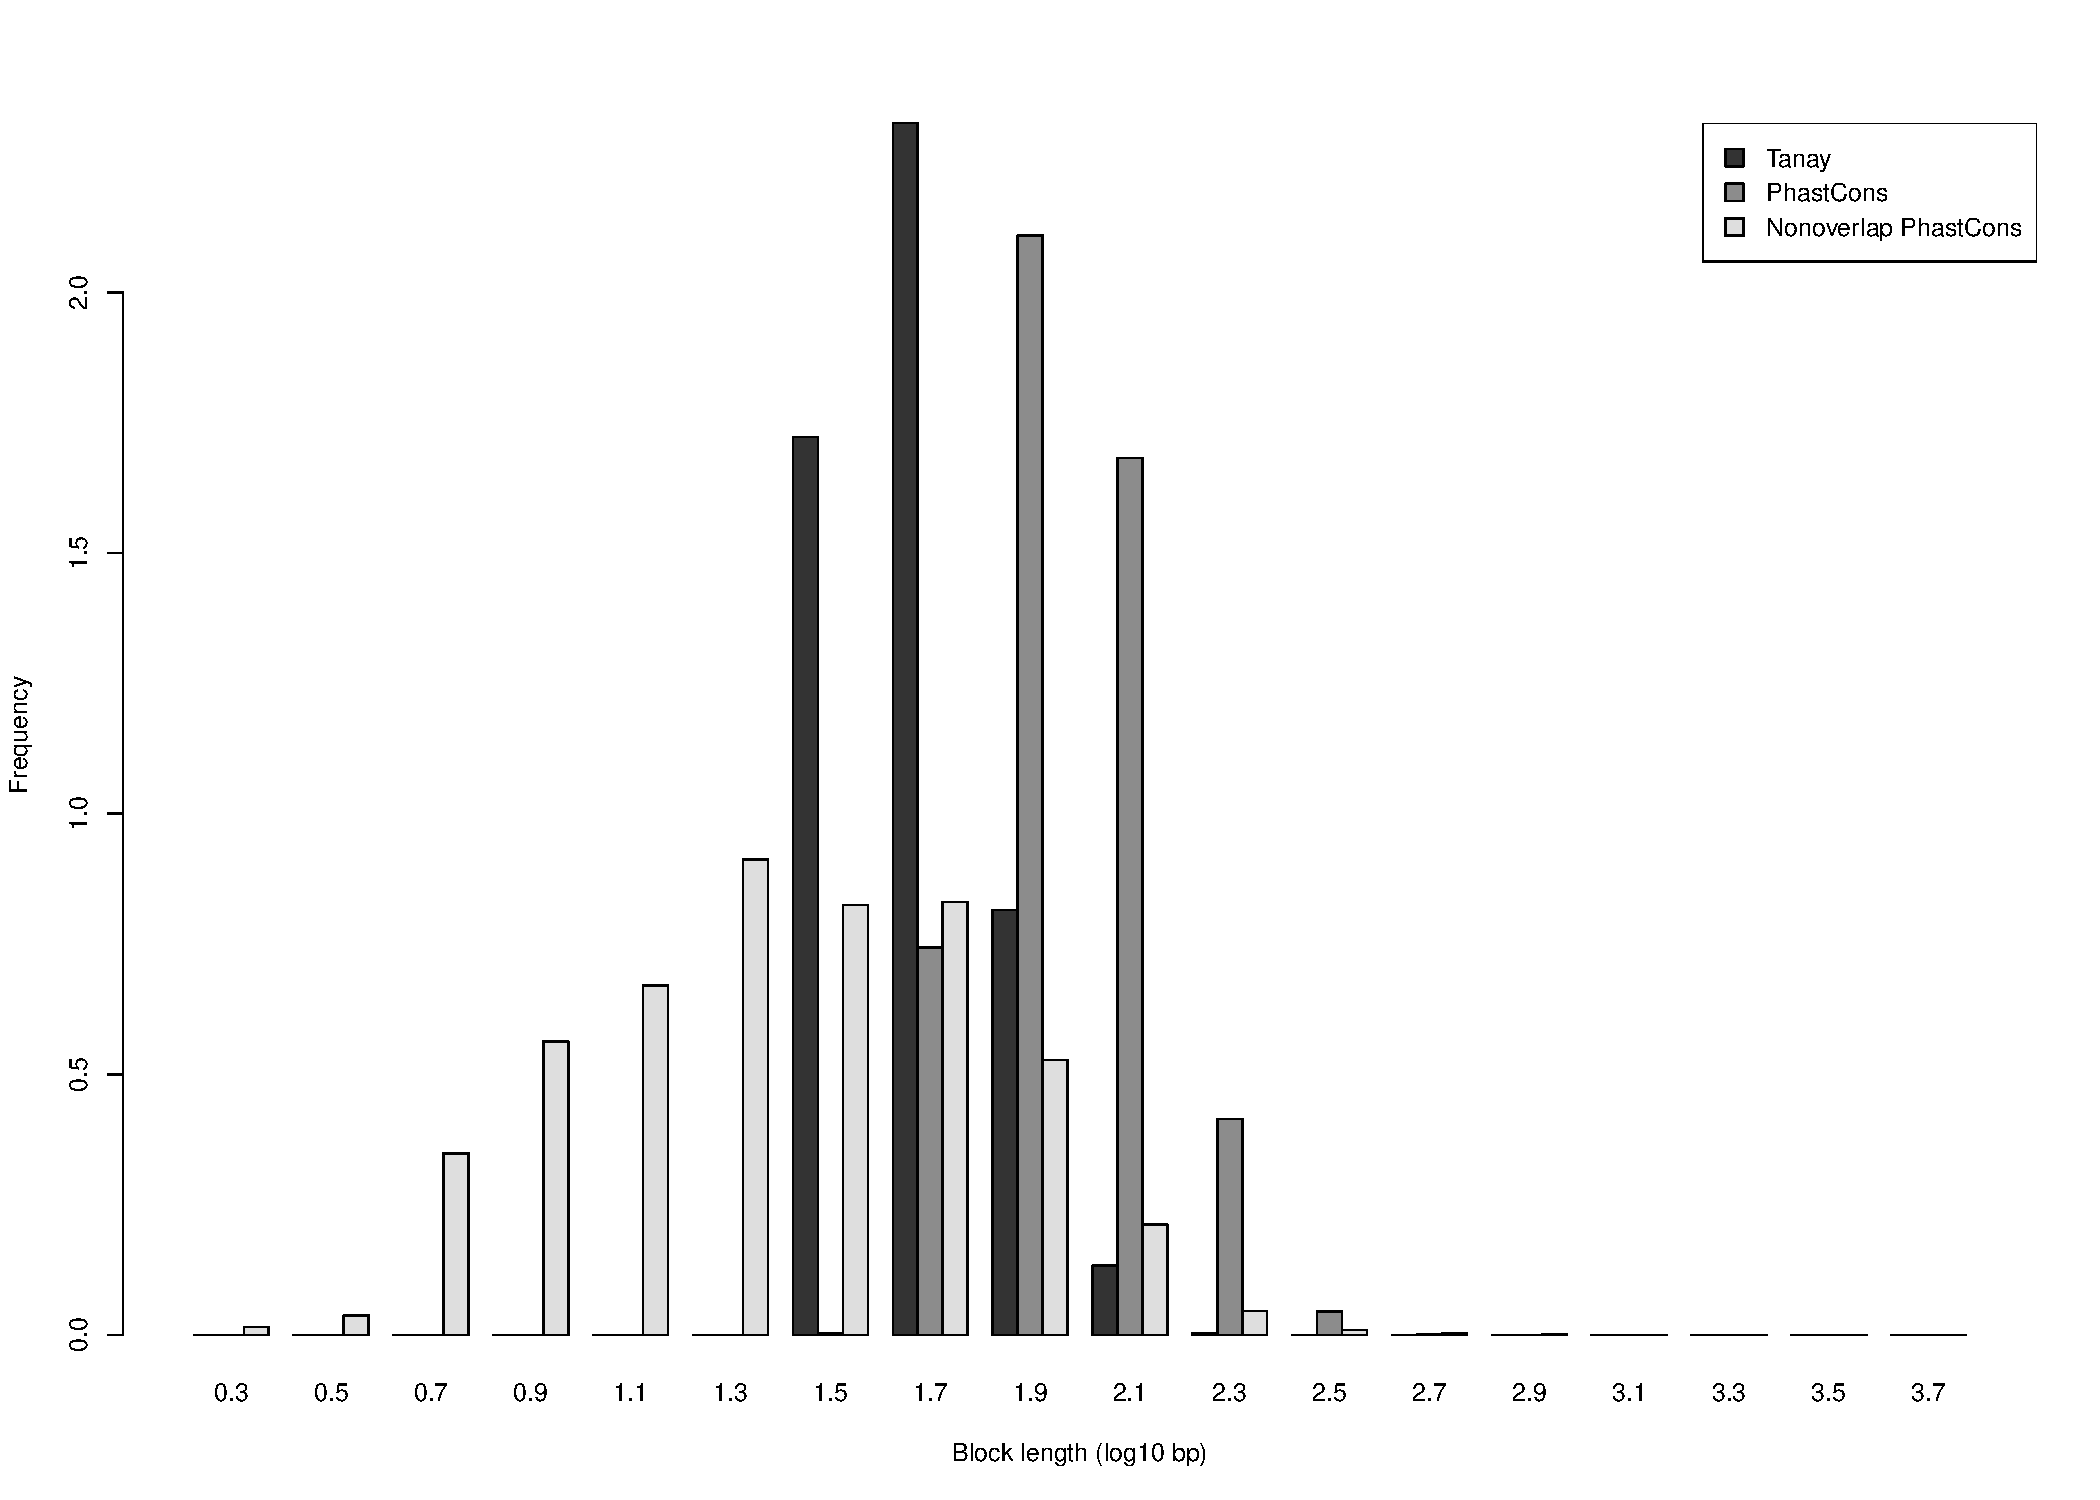
\includegraphics[width=\textwidth, height=85mm]{hists_side_by_side}}
\caption[Caption for LOF]{\centering Histogram of block lengths of 1:1 overlap Tanay and phastCons data sets, and nonexonic nonoverlapping phastCons data set.}
\label{fig:1_1_hists}
\end{figure}

\newpage
\subsection{Base composition analysis of nonexonic conserved elements}
The lengths of nonexonic conserved blocks and spacers were generated and calculated. The frequency of occurrence by classes of nonexonic blocks and spacers of Tanay and phastCons revealed significant different distributions (Figure 7). In addition, the lengths of phastCons blocks were found to be larger than Tanay (see left panel of Figure 7), and the lengths of Tanay spacers were found to be larger than phastCons spacers (see right panel of Figure 7). This study conducted a comprehensive base composition analysis of nonexonic blocks and spacers. This investigation included calculating the percentage of GC-content of blocks and spacers, and studying the side effects of CEs and the relationship between base composition and block length.

\subsubsection{GC-content}
The importance of studying base composition of CEs is to study the evolutionary forces that shape genomes. This investigation include a number of CE data sets: (i) 1:1 overlap data set between Tanay and phastCons CEs, (ii) phastCons CEs date set that do not overlap with Tanay CEs, and (iii) nonexonic CEs of Tanay and phastCons. The GC content of differnt CEs data sets was found to vary. For 1:1 overlap data set, the average of GC content of Tanay blocks (41.44\%) and phastCons blocks (42.25\%) was compared to the GC content of Tanay spacers (42.72\%) and phastCons spacers (42.77\%) (Figure 7). For Tanay and phastCons data sets, sequences of spacer were found to be more GC-rich than sequences of blocks. In addition to blocks and spacers of 1:1 overlap data set, average of GC-rich sequences that flank the larger conserved blocks (phastCons blocks) were shown to increase to 43.28\% (Figure 8).\\\\  
Similarly, for phastCons blocks that do not overlap with Tanay blocks (nonoverlap data set), average of spacers were found to include more GC-rich sequences (42.83\%) than block sequences (42.37\%), (see right panel of Figure 9). For all nonexonic conserved elements of Tanay and phastCons, average of spacer sequences of Tanay and phastCons (42.72\% and 42.95\%, respectively) are more GC-rich than sequences of Tanay blocks (41.45\%) and phastCons blocks (42.36\%) (see left and middle panels of Figure 9).\\

\begin{figure}[htbp]
\centering
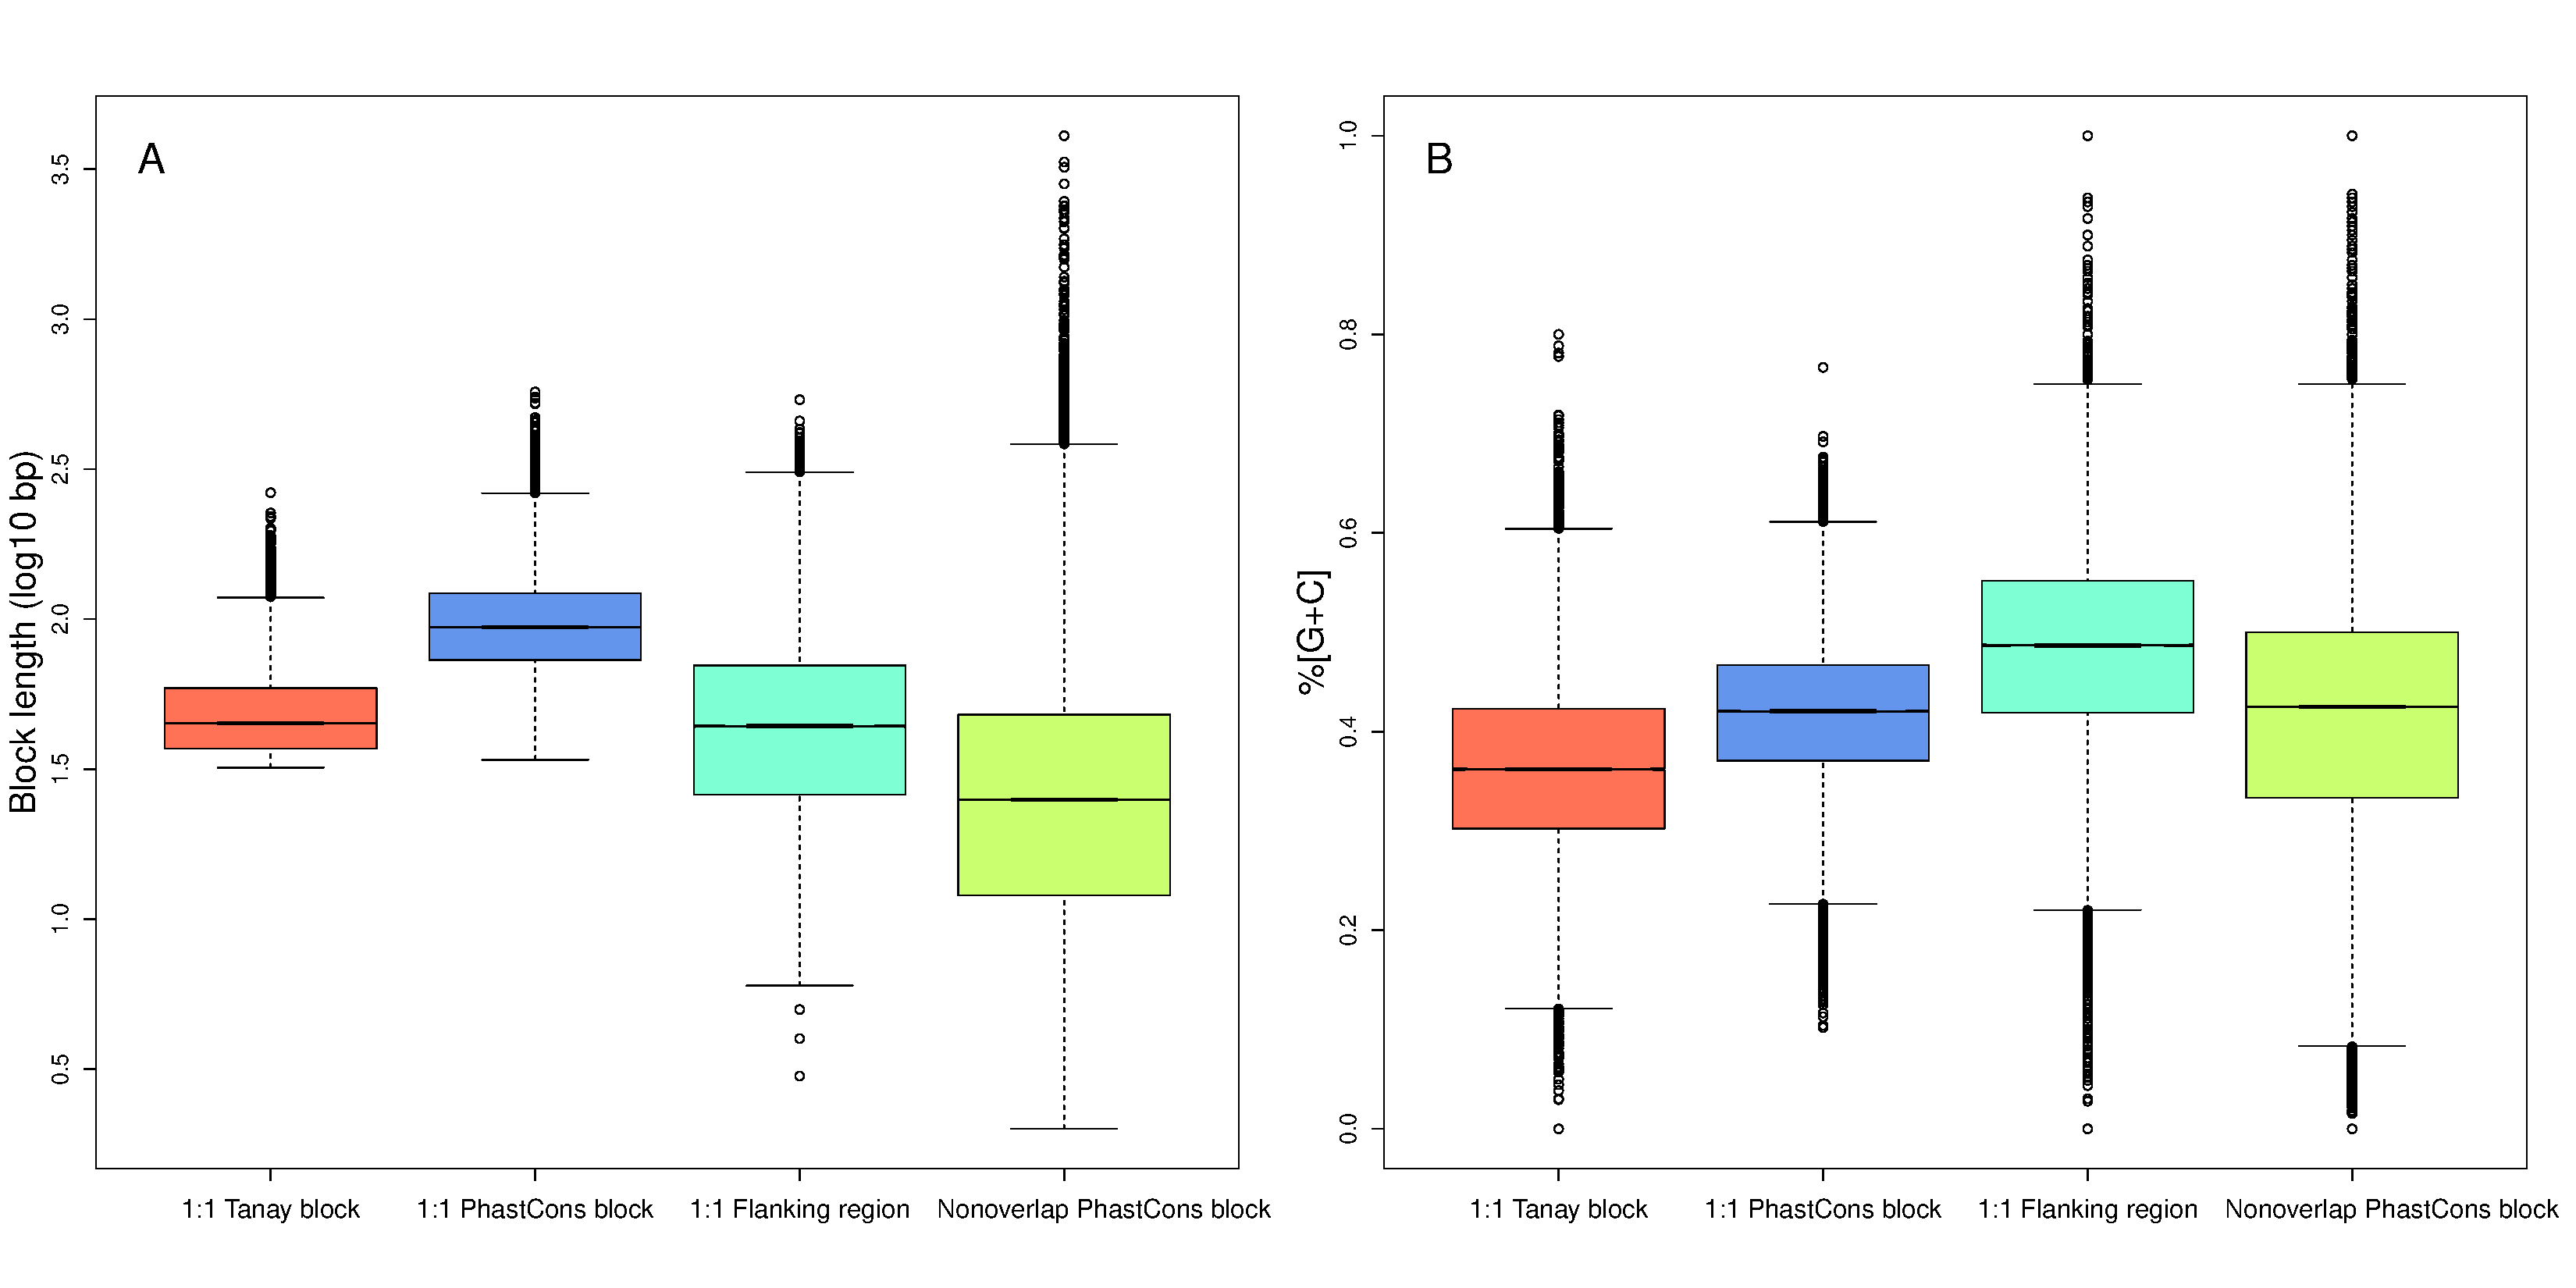
\includegraphics[width=\textwidth, height=82mm]{nonexonic_1_1_GC_lengths}
\caption{The box plots show lengths (left panel) and average GC content (right panel) of 1:1 data sets for blocks and spacers of Tanay and phastCons, and sequences flanking the larger conserved blocks.}
\label{fig:1_1_base_comp}
\end{figure}

\begin{table}[ht]
\centering
\begin{tabular}{c c c}
\hline\hline
\ Data set & Average length (bp) & Average GC\% \\ [0.5ex]
\hline
1:1 Tanay blocks & 46.9 & 0.363 \\
1:1 PhastCons blocks & 94.9 & 0.417 \\
1:1 Flanking region & 49.6 & 0.483 \\
Nonoverlap PhastCons blocks & 33.7 & 0.420 \\ [1ex]
\hline
\end{tabular}
\caption[Caption for LOF]{\centering Average lengths and GC content of 1:1 data sets.}
\end{table}

\begin{figure}[htbp]
\centering
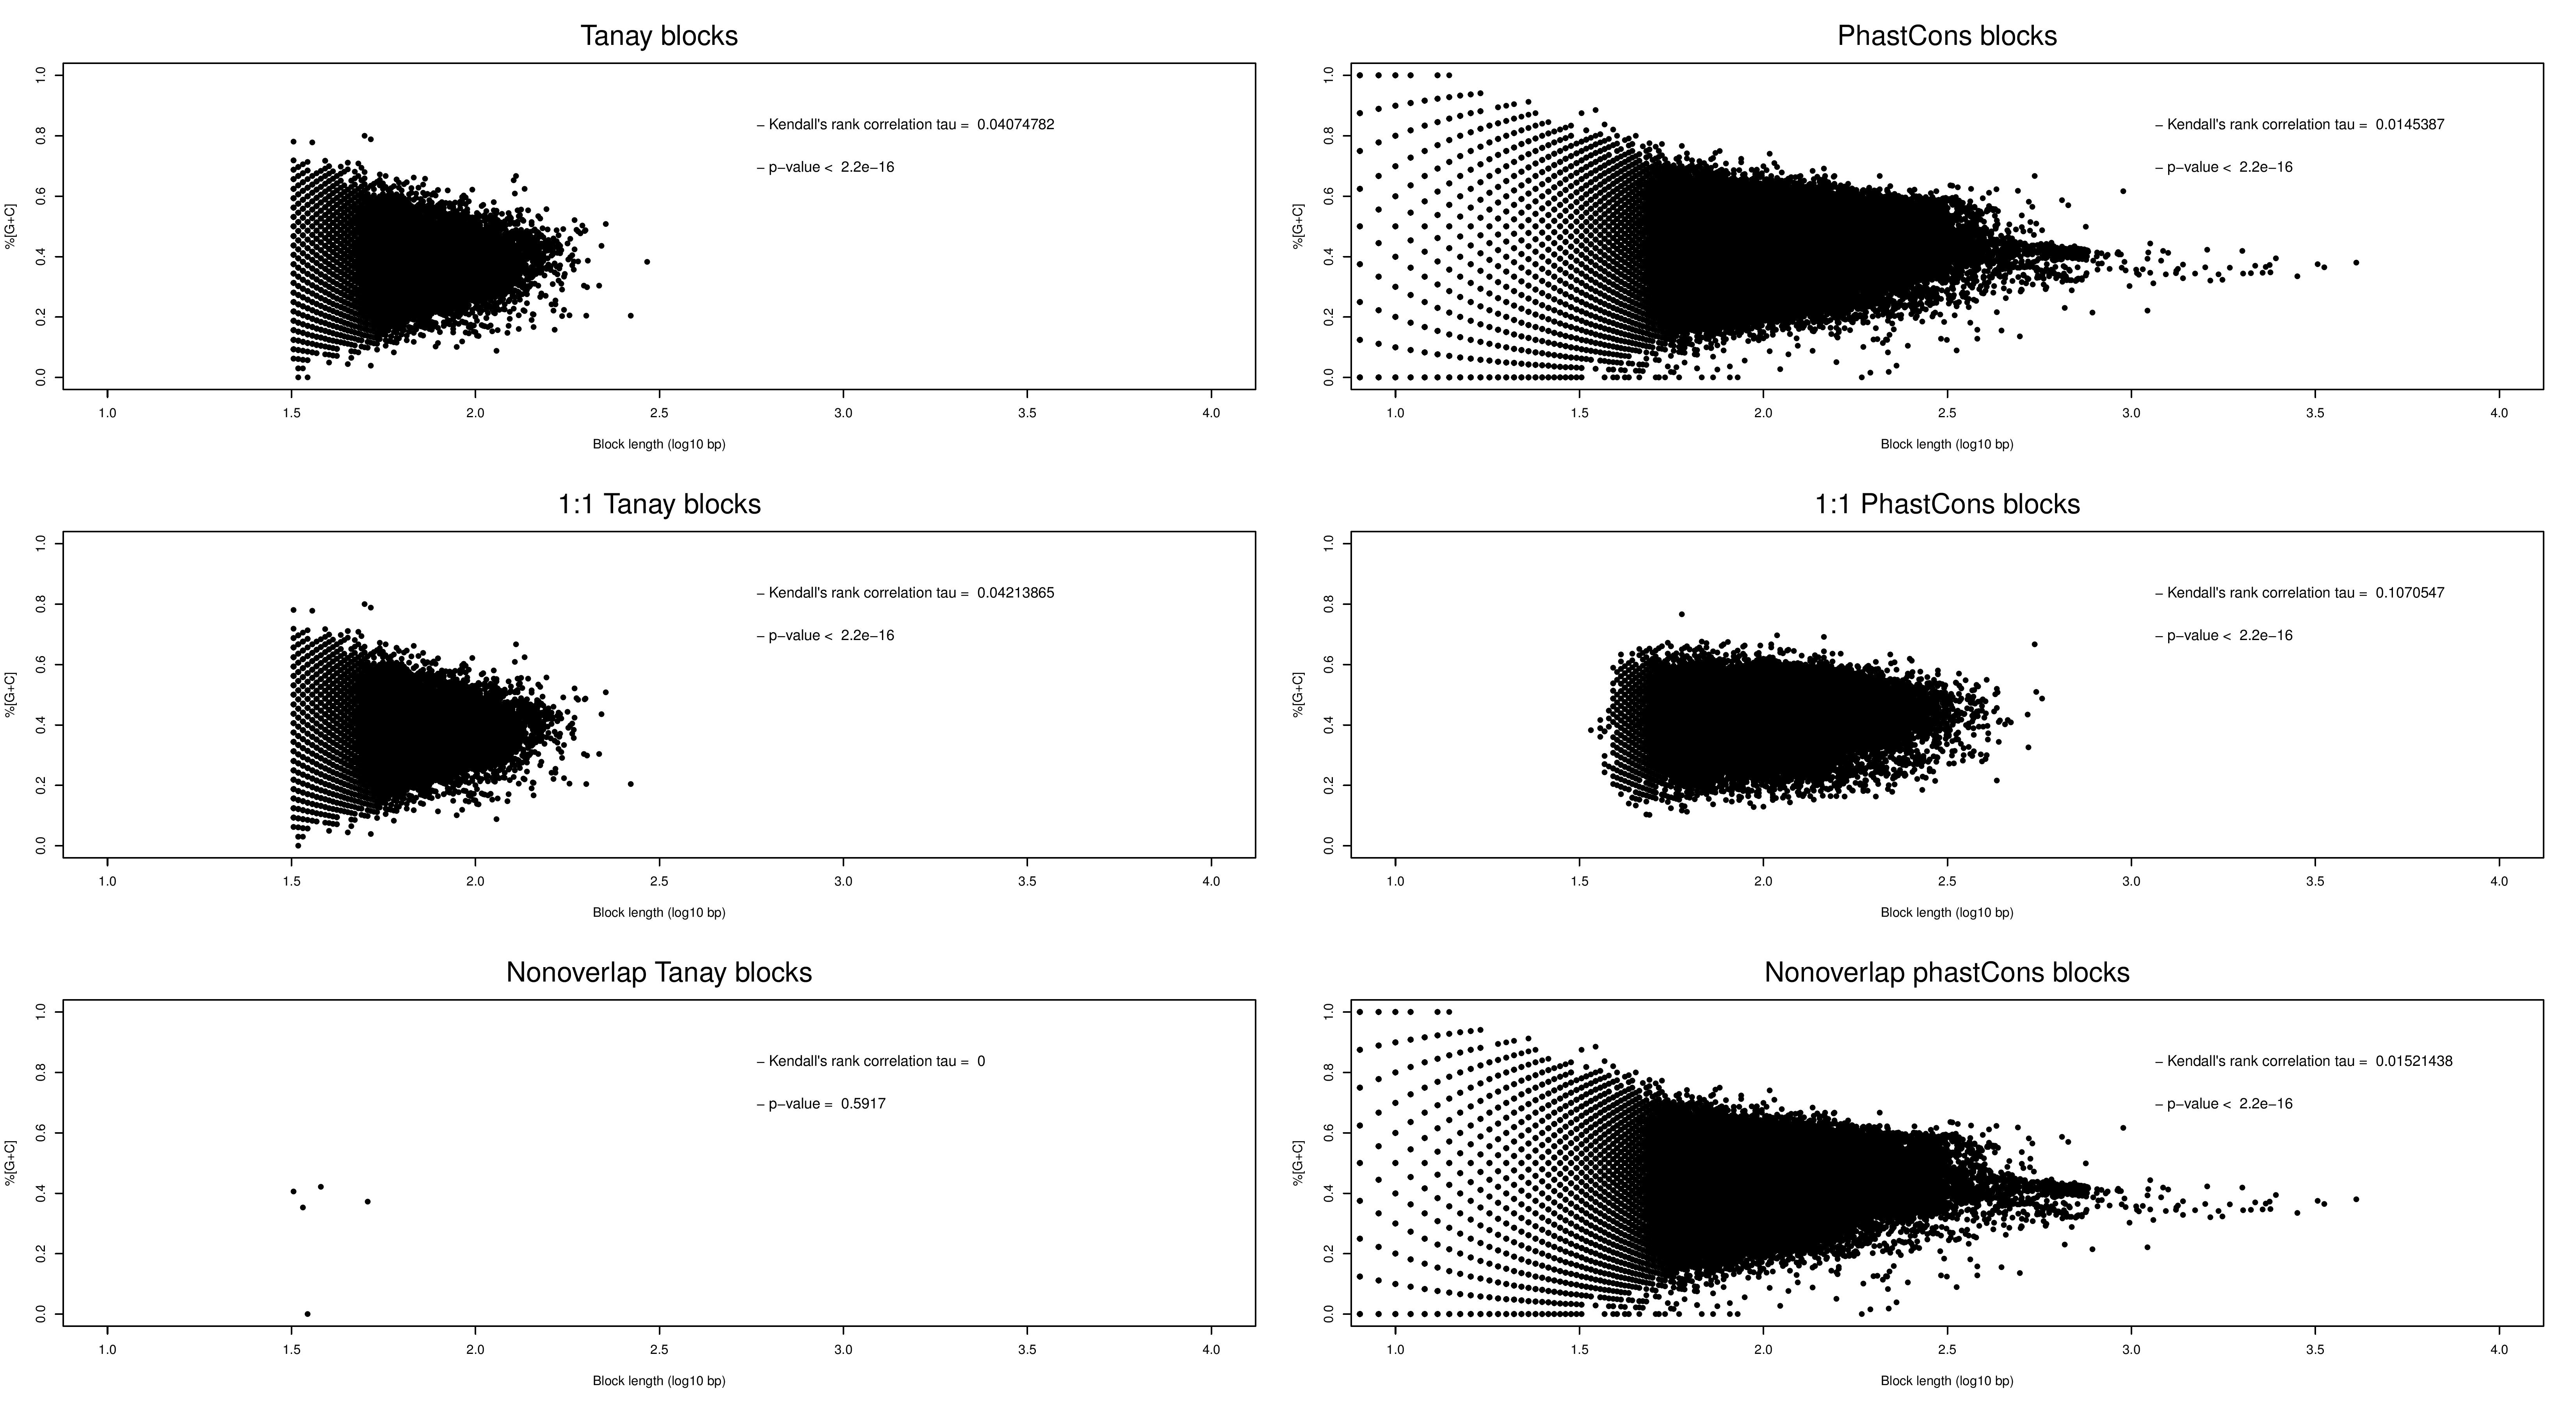
\includegraphics[width=\textwidth, height=92mm]{all_length_vs_GC_scatterplots.jpg}
\caption{The scatter plots show the relationship between GC content and block length for nonexonic Tanay and phastCons blocks (first row), 1:1 overlap Tanay and phastCons blocks (second row), and nonexonic nonoverlapping Tanay and phastCons blocks (third blocks).}
\label{fig:scatter_all}
\end{figure}

\subsubsection{Side effects of conserved elements}
Kenigsberg and Tanay found that CEs (Tanay blocks) have typically high AT content and high GC content levels around these elements \citep{Tanay2013}. They found, in particular, a sharp increase of GC-rich regions of DNA around the edges of CEs. Additionally, GC profile around CEs was not symmetrical. In a previous investigation, almost all Tanay blocks were found to overlap with phastCons blocks. This raises the hypothesis that the side effects are artifact of incomplete definition of Tanay conserved blocks. This hypothesis led to the decision that we needed to perform base composition for regions flanking the CEs. Tanay, phastCons, 1:1 overlap and nonoverlap data sets were included to investigate the side effects of CEs. ATGC profiles were generated to plot the base composition of regions flanking CEs over two distance scales (1 kb and 100 bp), starting from two start points: (i) the edge-point of CEs, and (ii) the mid-point of CEs.\\\\
For 1:1 overlap data set, ATGC profiles were plotted for overlapping blocks of Tanay and phasCons (Figure 10). ATGC profiles significantly extended the previous study \citep{Tanay2013}. For the edge-point case of both Tanay and phastCons CEs, there was an obvious increase of GC content in the regions around CEs (see bottom Figures of a10). For the mid-point case of both Tanay and phastCons CEs, there was an increase of GC content in the regions around the CEs followed by a sharp AT increase at the CE borders (see bottom Figures of b10).\\\\ 
These observations led to the conclusion that ATGC profiles of nonoverlap phastCons blocks were required to be generated. For the edge-point case, there were an increase of GC content and decrease of AT content (see right Figures of 12). However, the level of AT content were shown to be higher than GC content. For the mid-point case, there were a slight increase of GC content and slight decrease of AT content (see left Figures of 12).\\\\  
Similarly, ATGC profiles were plotted for nonexonic CEs of Tanay and phasCons (Figure 11). For the edge-point case of Tanay CEs, as seen in 1:1 overlap data set, there was an obvious increase of GC content in the regions around CEs (see bottom-left Figure of a11). For the edge-point case of phastCons CEs, as seen in nonoverlap data set, there were an increase of GC content and decrease of AT content (see bottom-right Figure of a11). For the mid-point case of Tanay CEs, as seen in 1:1 overlap data set, there was an increase of GC content in the regions around the CEs followed by a sharp AT increase at the CE borders (see bottom-left Figure of b11). For the mid-point case of phastCons CEs, as seen in nonoverlap data set, there were a slight increase of GC content and slight decrease of AT content (see bottom-right Figure of b11).\\\\
The symmetry of the GC profiles around CEs was observed to be skewed. Furthermore, these investigations assumed that blocks identified independently of GC and that GC content is homogeneous within block. To study the effect of block length on GC profile, an investigation were required to address whether there is a relationship between base composition and block length or position in block.\\

\begin{figure}[htbp]
\centering
\frame{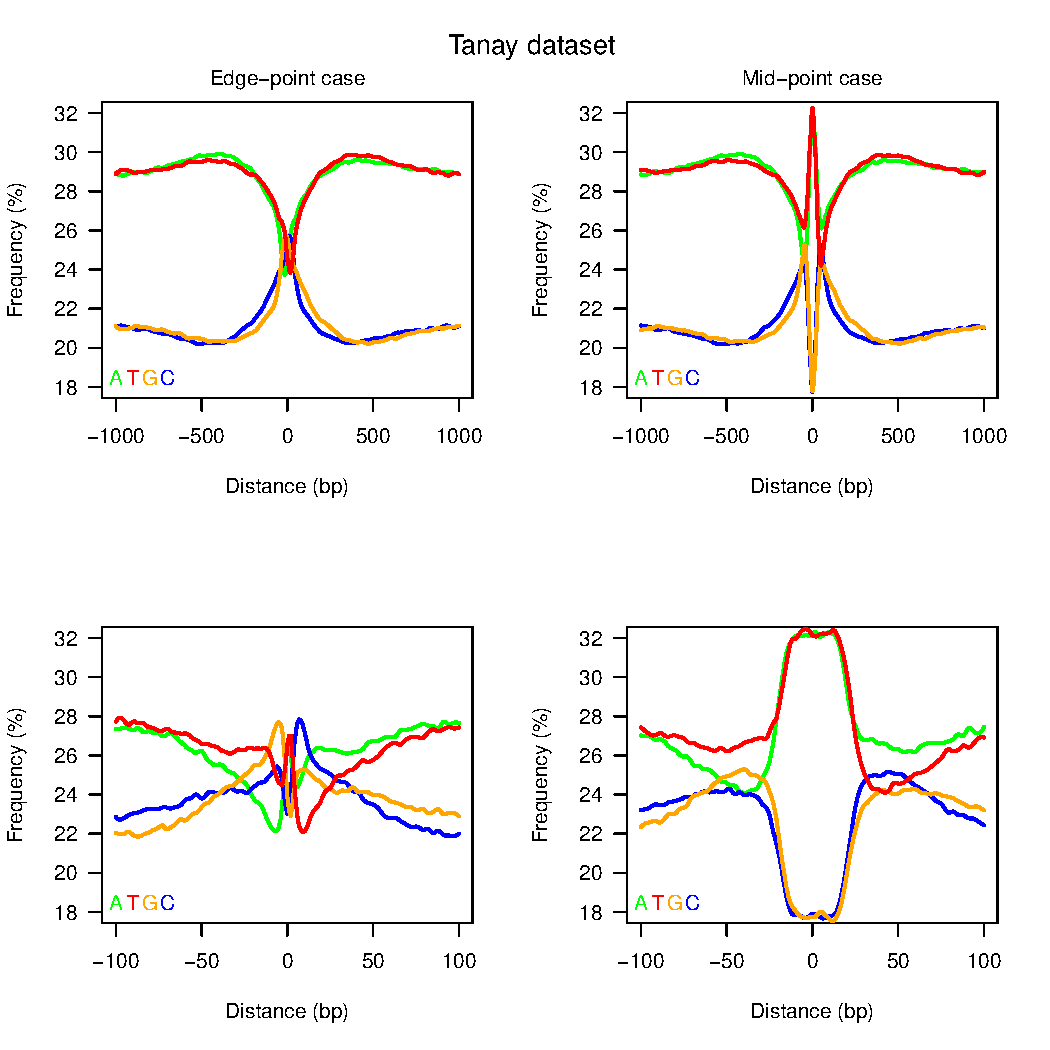
\includegraphics[width=\textwidth, height=120mm]{nonexonic_tanay_ATGC_profile}}
\caption{The percentage of ATGC profiles of nonexonic Tanay CEs are plotted over two distance scales (1 kb in top figures, 100 bp in bottom figures), starting from the edge-point of CEs (left figures), and the mid-point of CEs (right figures).}
\label{fig:ATGC_tan}
\end{figure}

\begin{figure}[htbp]
\centering
\frame{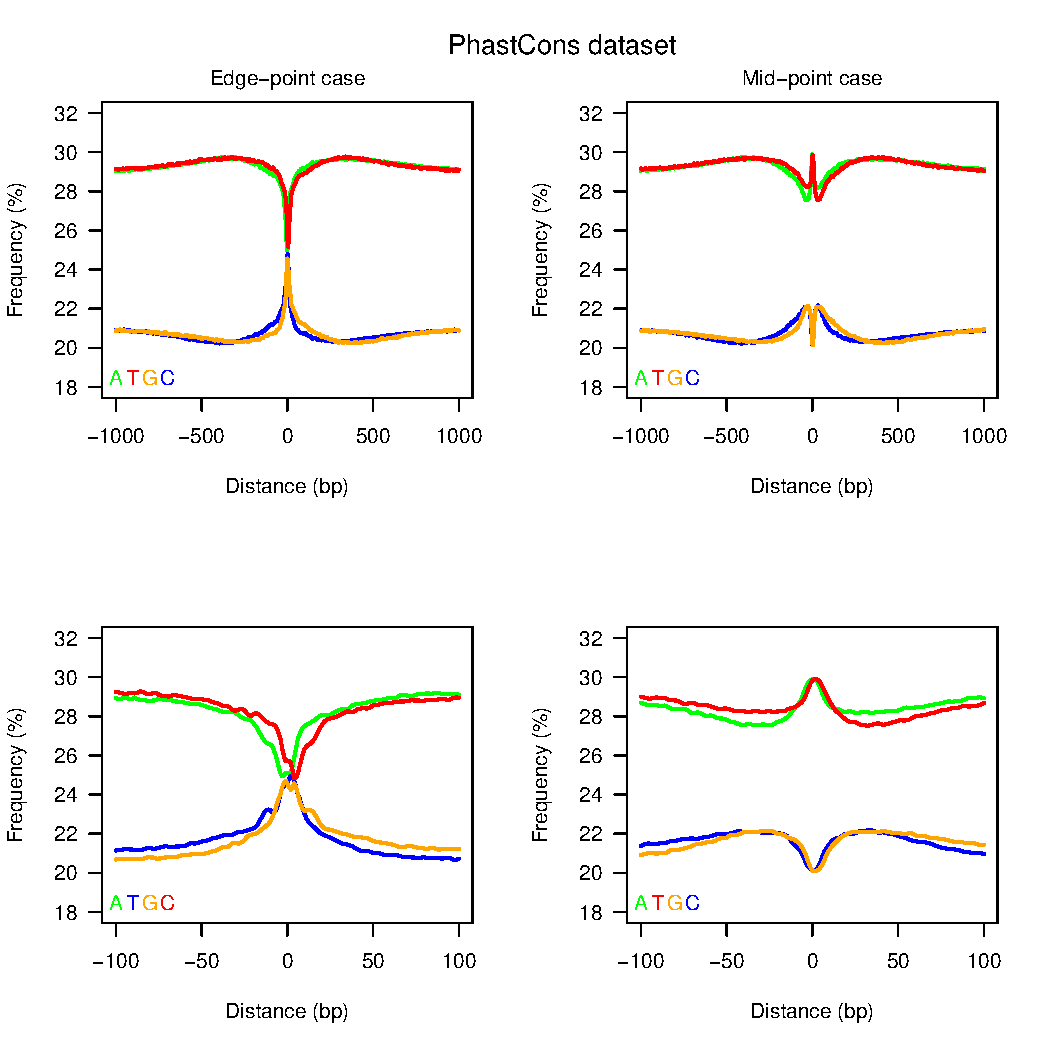
\includegraphics[width=\textwidth, height=120mm]{nonexonic_PC_ATGC_profiles}}
\caption{The percentage of ATGC profiles of nonexonic phastCons CEs are plotted over two distance scales (1 kb in top figures, 100 bp in bottom figures), starting from the edge-point of CEs (left figures), and the mid-point of CEs (right figures).}
\label{fig:ATGC_phast}
\end{figure}

\begin{figure}[htbp]
\centering
\frame{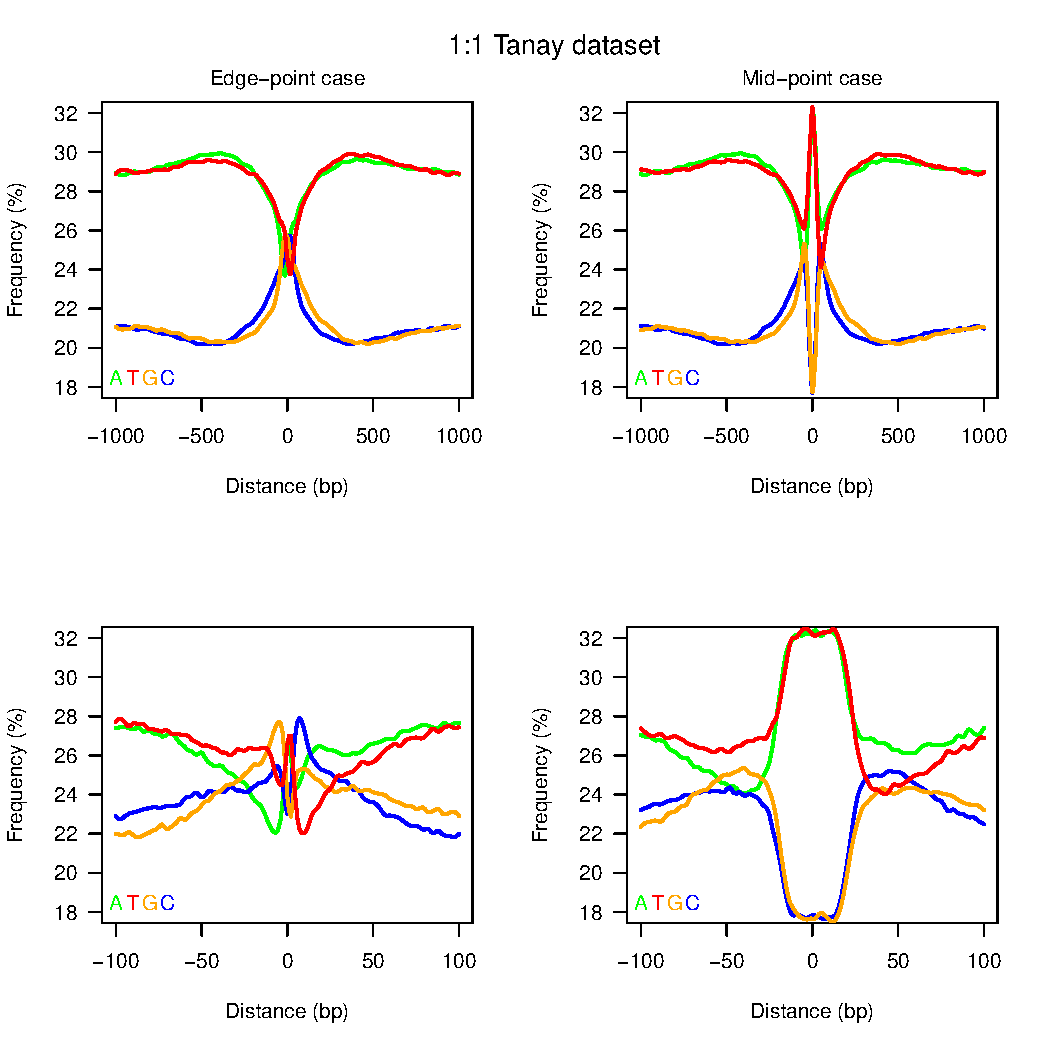
\includegraphics[width=\textwidth, height=120mm]{1_1_tan_ATGC_profile}}
\caption{The percentage of ATGC profiles of nonexonic Tanay CEs are plotted over two distance scales (1 kb in top figures, 100 bp in bottom figures), starting from the edge-point of CEs (left figures), and the mid-point of CEs (right figures).}
\label{fig:ATGC_1_1_tan}
\end{figure}

\begin{figure}[htbp]
\centering
\frame{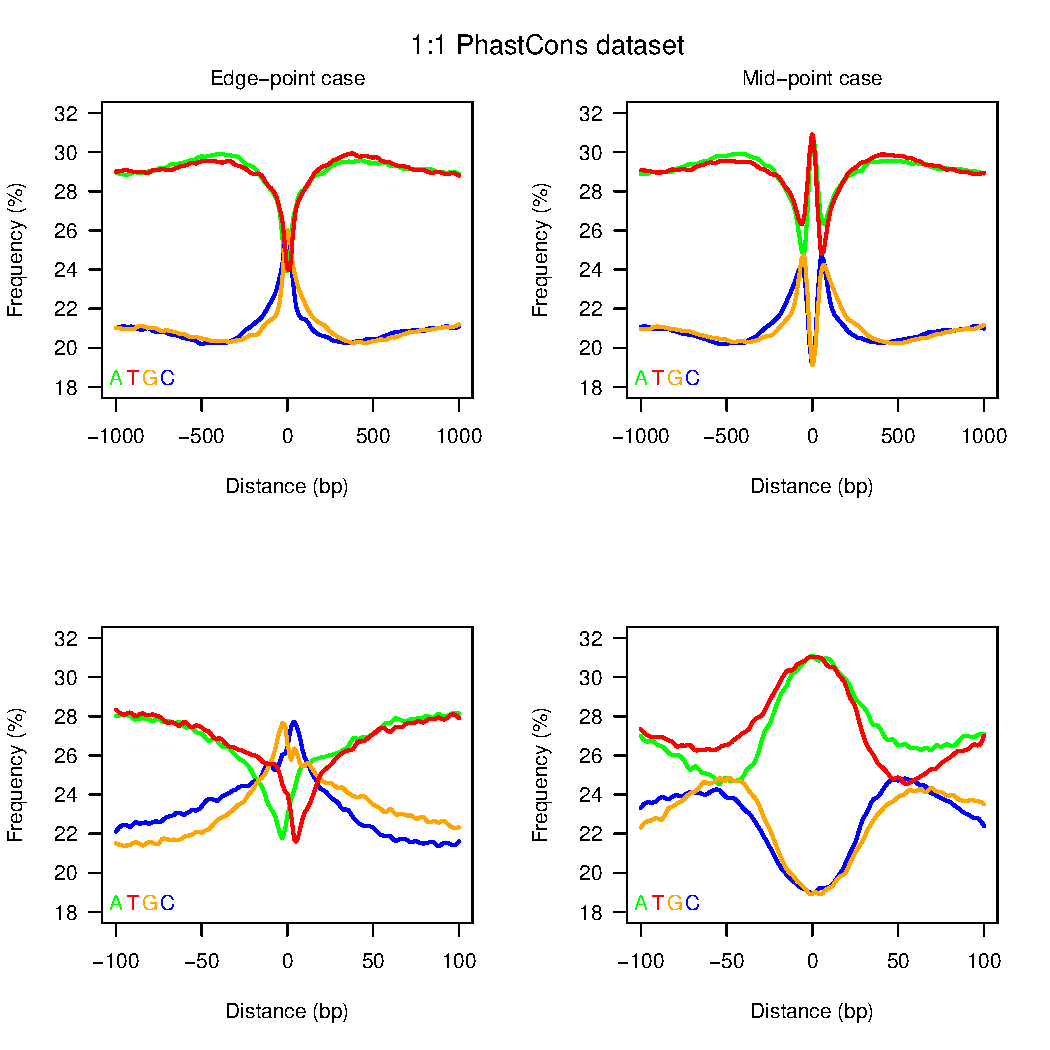
\includegraphics[width=\textwidth, height=120mm]{1_1_phast_ATGC_profile}}
\caption{The percentage of ATGC profiles of nonexonic 1:1 phastCons CEs are plotted over two distance scales (1 kb in top figures, 100 bp in bottom figures), starting from the edge-point of CEs (left figures), and the mid-point of CEs (right figures).}
\label{fig:ATGC_1_1_phast}
\end{figure}

\begin{figure}[htbp]
\centering
\frame{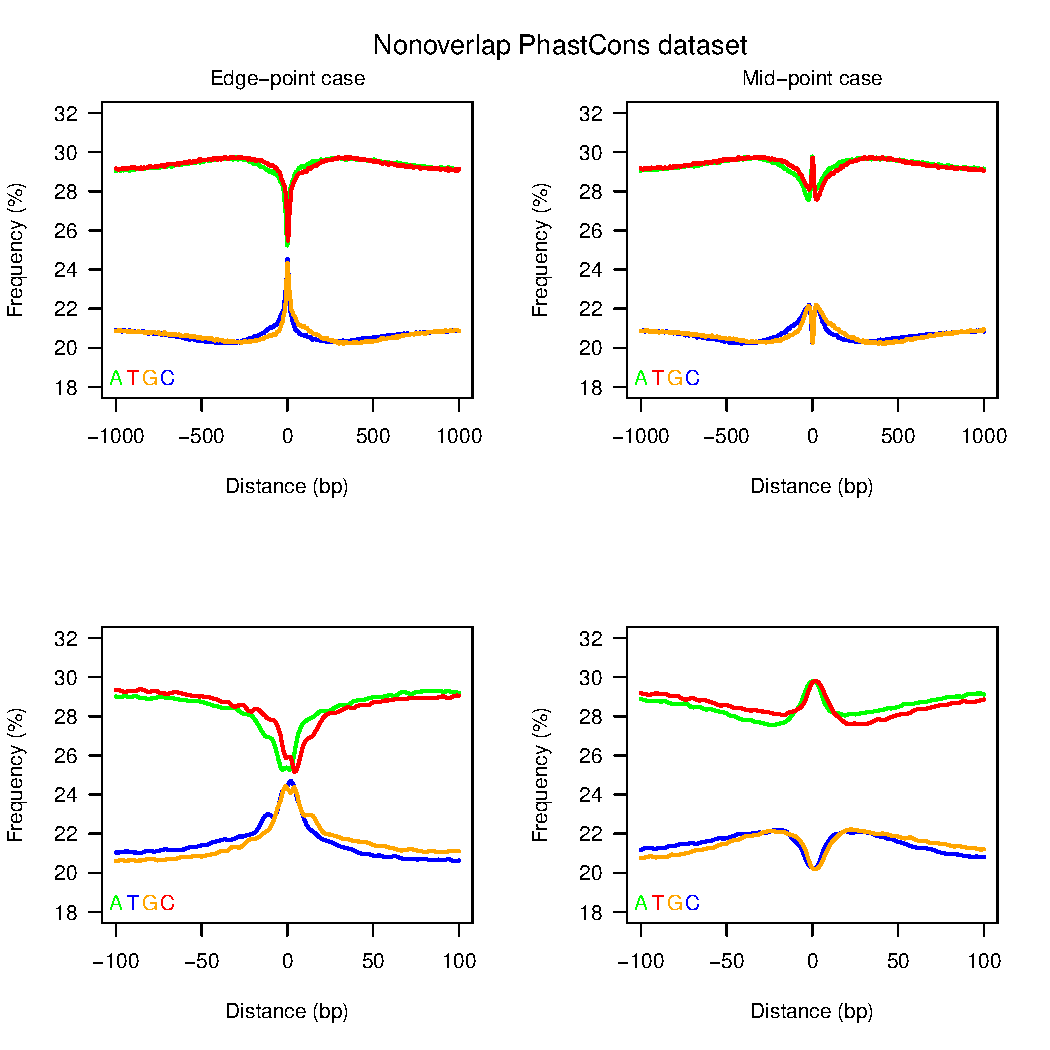
\includegraphics[width=\textwidth, height=120mm]{nonexonic_nonoverlap_PC_ATGC_profiles}}
\caption{The percentage of ATGC profiles of nonexonic nonoverlapping phastCons CEs are plotted over two distance scales (1 kb in top figures, 100 bp in bottom figures), starting from the edge-point of CEs (left figures), and the mid-point of CEs (right figures).}
\label{fig:nonoverla_ATGC}
\end{figure}

\begin{figure}[htbp]
\centering
\frame{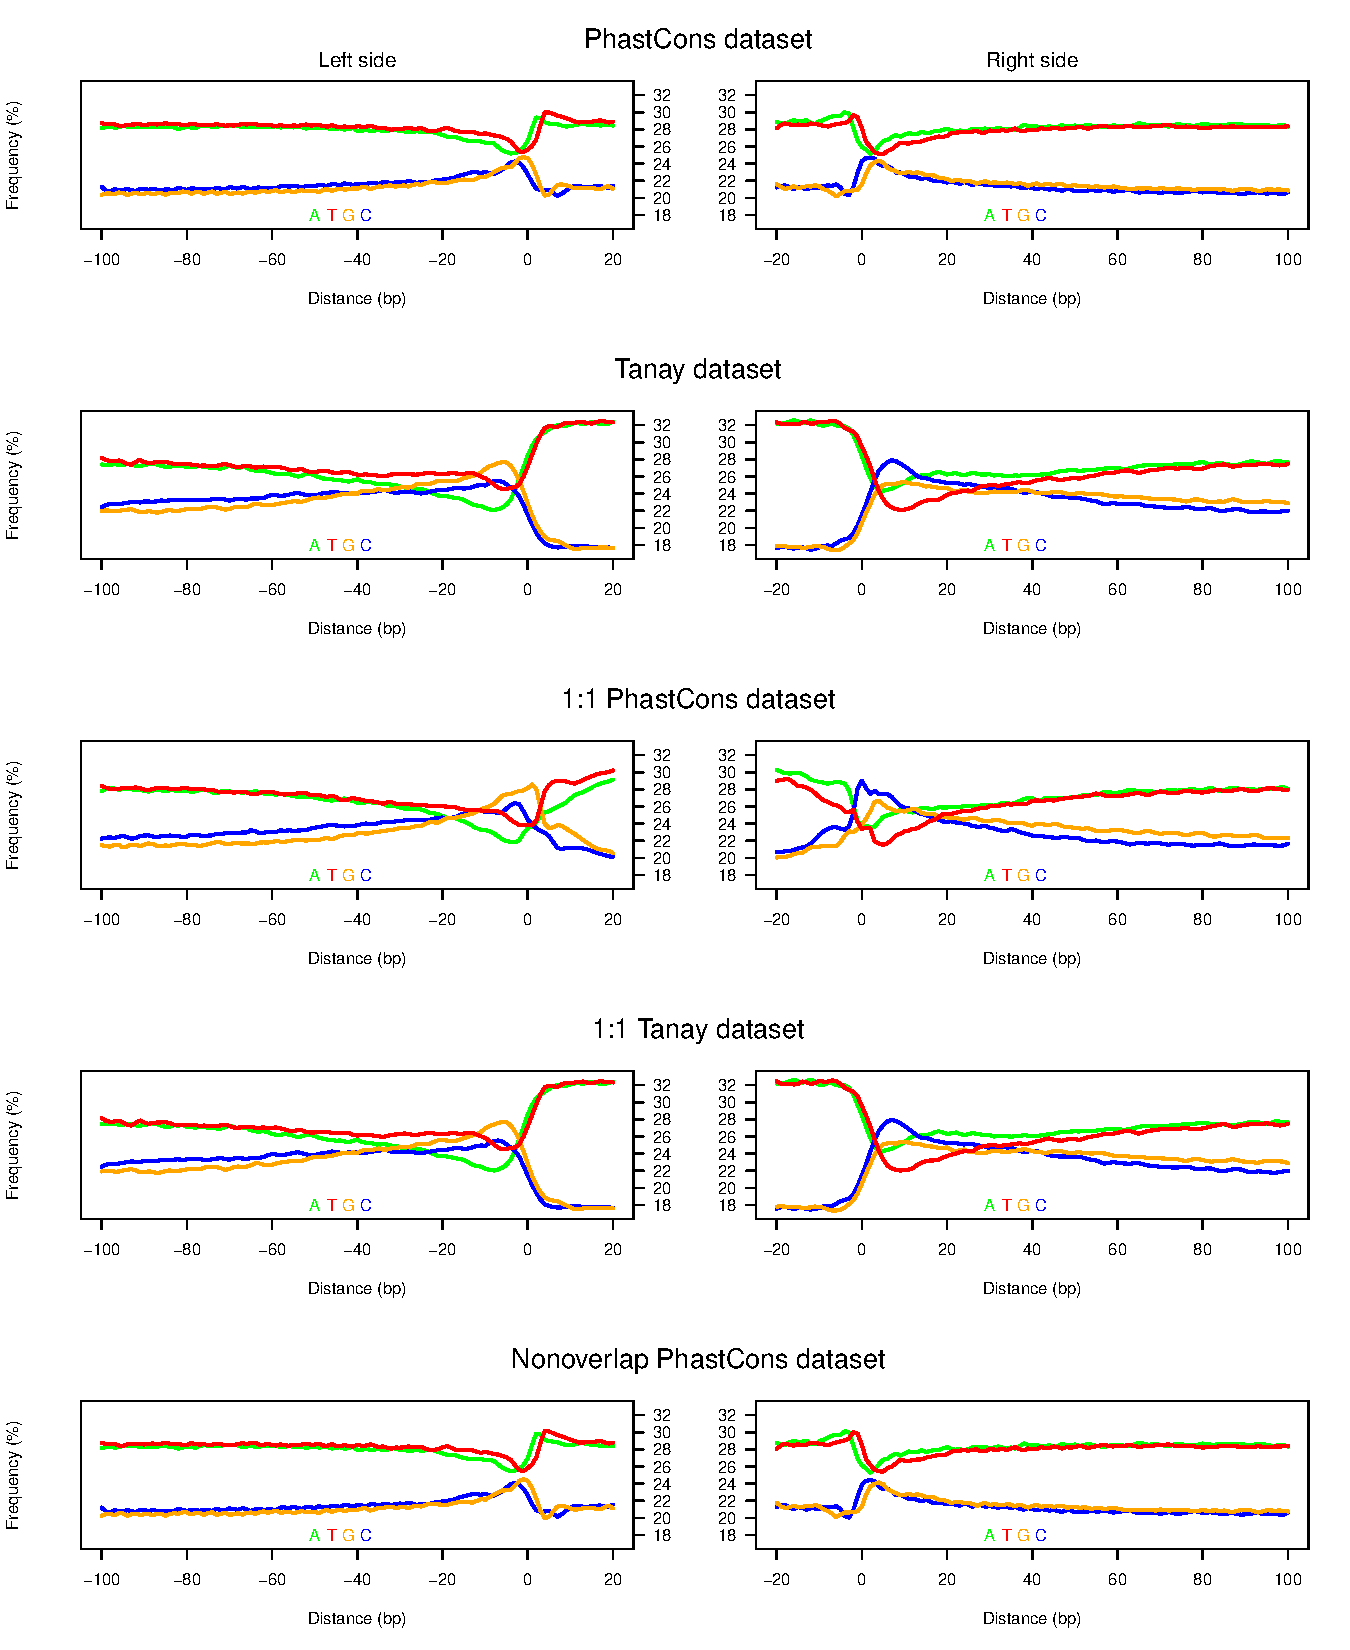
\includegraphics[width=\textwidth, height=140mm]{aligned_ATGC_profiles}}
\caption{The percentage of ATGC profiles are plotted for 100 bp of sequence flanking CEs and 20 bp of CEs at the CEs border of left side (left figures) and  right side (right figurs) for nonexonic phastCons data set(first row), nonexonic Tanay data set (second row), nonexonic 1:1 phastCons data set (third row), nonexonic Tanay data set (fourth row) and nonexonic nonoverlapping phastCons data set (fifth row).}
\label{fig:aligned_all}
\end{figure}

\newpage 
\bibliographystyle{plainnat}
\bibliography{eng_manee}
\end{document}
                      